%% LyX 2.0.0 created this file.  For more info, see http://www.lyx.org/.
%% Do not edit unless you really know what you are doing.
\documentclass[11pt,english,preprint]{aastex}
\usepackage[T1]{fontenc}
\usepackage[latin9]{inputenc}
\setcounter{tocdepth}{3}
\usepackage{graphicx}

\makeatletter
%%%%%%%%%%%%%%%%%%%%%%%%%%%%%% User specified LaTeX commands.

%\documentclass[11pt,preprint]{/Users/js/words/aastex52/aastex}
\textwidth=6.8in
\textheight=9.2in
\oddsidemargin=-0.3in
\evensidemargin=-0.3in
\usepackage{epsfig}

\def\etal{\it et al. \rm }


\makeatother

\usepackage{babel}
\begin{document}

\title{ARCHANGEL Galaxy Photometry System}


\author{James Schombert}


\affil{Department of Physics, University of Oregon, Eugene, OR 97403; js@abyss.uoregon.edu}
\begin{abstract}
\noindent Photometry of galaxies has typically focused on small, faint
systems due to their interest for cosmological studies. Large angular
size galaxies, on the other hand, offer a more detailed view into
the properties of galaxies, but bring a series of computational and
technical difficulties that inhibit the general astronomer from extracting
all the information found in a detailed galaxy image. To this end,
a new galaxy photometry system has been developed (mostly building
on tools and techniques that have existed in the community for decades)
that combines ease of usage with a mixture of pre-built scripts. The
audience for this system is a new user (graduate student or non-optical
astronomer) with a fast, built-in learning curve to offer any astronomer,
with imaging data, a suite of tools to quickly extract meaningful
parameters from decent data. The tools are available either by a client/server
web site or by tarball for personal installation. The tools also provide
simple scripts to interface with various on-line datasets (e.g. 2MASS,
Sloan, DSS) for data mining capability of imaged data.

\noindent As a proof of concept, we preform a re-analysis of the 2MASS
Large Galaxy Atlas to demonstrate the differences in an automated
pipeline, with its emphasis on speed, versus this package with an
emphasis on accuracy. This comparison finds the structural parameters
extracted from the 2MASS pipeline is seriously flawed with scale lengths
that are too small by 50\% and central surface brightness that are,
on average, 1 to 0.5 mags too bright. A cautionary tale on how to
reduce information-rich data such as surface brightness profiles.
This document and software can be found at http://abyss.uoregon.edu/$\sim$js/archangel.
\end{abstract}

\section{Introduction}

The photometric analysis of large galaxies is a double edged sword.
While increased resolution, compared to distant galaxies, provides
avenues for more detailed analysis of galaxy properties (to name a
few: examination of star formation regions, examination of core parameters
to search for massive blackholes, spiral arm analysis, isophotal irregularities
that may signal rings, bars or other secular evolution processes),
it is a data reduction fact that the larger number of pixels complicates
the extraction of simple parameters, such as total magnitude, mean
surface brightness and isophotal radius. For example, the fact that
the galaxy is spread over a larger area of the sky means that the
outer pixels have more sky luminosity than galaxy luminosity, increasing
the error in any galaxy value. In addition, increased angular size
has frequently prevented a fair comparison between distant and nearby
galaxy samples simply because the techniques used to extract parameters
from nearby galaxies differ from those used on small galaxies.

In general, the analysis of large galaxies (i.e. ones with many pixels)
requires a full surface photometry study of the isophotes and their
shape. For most extragalactic systems, the shape of choice is an ellipse.
The astrophysics behind this assumption is that galaxy light traces
stellar mass, and stellar mass follows elliptical orbits as given
by Kepler's 1st law. Certainly, this is true the case of early-type
galaxies (elliptical and S0's) as demonstrated by studies that examined
the residuals from elliptical isophotes (Jedrzejewski 1987). This
is also mostly true for disk galaxies, although the lumpiness of their
luminosity distribution due to recent star formation increases the
noise around each ellipse (see the discussion in \S 2.4). For dwarf
irregular systems, any regular contours are poor describers of their
shape, thus an ellipse is used because it is the simplest shape (aside
from a circle) to describe an irregular isophote.

Therefore, the analysis of large galaxies begins with the reduction
of their 2D images into 1D surface photometry as described by elliptical
isophotes. In turn, the 1D profiles can be fit to various functions
in order to extract characteristic luminosities (stellar mass), scale
lengths and standard surface brightnesses (luminosity density). When
combined with kinematic information, these three parameters form the
Fundamental Plane for galaxies, a key relationship for understanding
the formation and evolution of galaxies.

Aside from direct relevance to the Fundamental Plane, the need for
better galaxy photometric tools has also increased with the influx
of quality HST imaging. Before HST, distant galaxies were mere point
sources, but now with WFPC2, ACS and NICMOS data, there is the need
to perform full surface photometric studies on a much larger volume
of the Universe. The sizes of our database on the photometric structure
of galaxies has increased a thousandfold in the last 10 years, but
most of the tools used to reduce this new data are up to 20 years
out-of-date. Thus, the analysis of high resolution space imaging data
is far behind spectroscopic and high energy data, not due to lack
of interest, but due to the inadequacy of our 2D analysis tools.

The goal of this software project (called the ARCHANGEL project for
obtuse historical reasons) has been to produce a series of proto-NVO
type tools, related to surface photometry, and develop a computing
environment which will extend the capability of individual observers
(or entire data centers) to perform virtual observatory science. There
is no attempt herein to replace existing analysis packages (i.e. PyIRAF),
but rather our goal is to supplement existing tools and provide new
avenues for data reduction as it relates to galaxy photometry. We
hope that the fundamental components in this package will provide
the community with new methods to which they can add their own ideas
and techniques as well as provide learning environment for new researchers.
In addition, there is growing amount of data by non-optical astronomers
as new space missions provide imaging data in wavelength regions previously
unexplored. Thus, there is a new and growing community of non-optical
astronomers with 2D analysis needs that we hope to serve.


\section{Package Philosophy}

The tools described herein are not intended to be a complete data
reduction package per say, but rather a set of basic modules that
allows the user to 1) learn the procedures of galaxy photometry, 2)
tailor the tools to their particular needs, 3) begin an advanced learning
curve of combining basic modules to produce new and more sophisticated
tools. Turning raw data (level 1 or 2 data) from the telescope (space
or ground) into calibrated, flattened images is the job of other,
more powerful packages such as PyRAF. The tools presented herein bridge
the intermediate step between calibrated data and astrophysically
meaningful values. Specifically, we are concerned with the analysis
of 2D images into 1D values, such as a surface brightness profile,
and further tabulation into final values, such as total luminosity
or scale length.

With respect to galaxy images, the numbers most often valued are luminosity,
scale length and luminosity density. Unfortunately, due to the extended
nature of galaxies, the quality and accuracy of these values can varying
depending on the type of value desired. For example, luminosities
can be extracted in metric form (luminosity within 16 kpc) or isophotal
(luminosity inside the 26.5 mag arcsecs$^{-2}$ isophote or the total
luminosity, an extrapolation to infinite radius. Scale length can
be expressed as the radius of half-light or a formula fit to the luminosity
distribution (e.g. Sersic function). Luminosity density can be described
through a detailed surface photometry profile, or integrated as a
mean surface brightness within an isophote, or again a fitted curve
such as an exponential disk. The tools provided by this project allow
an inexperienced user the capability to explore their dataset and
extract meaningful results while outlining the limitations to that
data.

For the experienced researcher, these tools enhance their previous
background in data reduction and provide new, and hopefully, faster
avenues of analysis. To this end, the tools provided by this package
provide a user with most basic of descriptions of a galaxy's light,
then allowing the option to select any meaningful parameter by toggling
a switch. For most parameters, such as aperture magnitudes, the switch
is simple and automatic. For more complicated parameters, such as
a profile fit or an asymptotic magnitude, the switch is understandably
more sophisticated and needing more explanation to the user for accurate
use.


\subsection{Basic Steps}

This paper is divided into five sections describing the major components
of the reduction package: 1) sky determination, 2) 2D profile fitting,
3) aperture photometry, 4) extraction of 1D parameters from surface
brightness profiles and 5) extracting total magnitudes. Each section
contains examples of the reduction of galaxy images from the 2MASS
archive.


\subsection{Quick Start}

The fastest way to introduce the techniques and tools used in our
package is to walk through the analysis of a several different types
of galaxy images. A more non-linear reader can refer to the Appendix
for a listing of the major tools. A script titled $profile$ is included
which outlines the usage of the routines described below. For a majority
of galaxy images, this script will produce a usable surface brightness
profile, and this script forms the core of the client/server version
of this package (see \S 5). But, a sharper understanding of the data
requires more interaction with the techniques, the user is encouraged
to run through the examples given in the package.

To illustrate our tools, we have selected 2MASS $J$ images of several
galaxies found in the Revised Shapley-Ames catalog with the characteristics
of smooth elliptical shape (NGC 3193), disk shape (IC 5271), spiral
features (NGC 157) and low in surface brightness/low contrast to sky
(NGC 2082). The analysis procedure for each galaxy is divided into
five basic parts; 1) sky determination, 2) cleaning, 3) ellipse fitting,
4) aperture photometry and 5) profile fitting.

Before starting it is assumed that the data frame has be initially
processed for flatfielding, dark subtraction and masking of chip defects.
Small defects, such as cosmic rays, are cleaned by the analysis routines.
But the errors are always reduced if known features are removed before
analysis. The following routines work on poorly flattened data (e.g.
gradients or large-scale features), and will signal the poorness by
the resulting errors, but the removal of large-scale flattening problems
requires more interaction then acceptable for this package and remains
the responsibility of the user.


\subsection{Sky Determination}

Any galaxy photometry analysis process begins with an estimate of
the image's sky value. While this is not critical for isophote fitting,
it is key for actually finding targets, cleaning the frame of stars
and smaller galaxies, plus determination of the photometry zeropoints.
Accurate sky determination will, in the end, serve as the final limit
to the quality of surface photometry data since a majority of a galaxy's
luminosity distribution is near the sky value. For this reason, sky
determination has probably received as much attention in astronomical
data literature as any other comparable reduction or analysis problem.

The difficulty in sky determination ranges from too few photons to
know the behavior of the instrumental response (e.g., high energy
data) to a high temporal varying flux of sky photons that overwhelms
the galaxy signal (e.g., near-IR data). Surface fitting, drift scans,
sky flats and super flats are all procedures used to minimize the
sky contribution to the noise levels of the final data. Several clever,
but not technically challenging, algorithms were included in the NOAO
IRAF system to handle time averaged flats and data, median co-adding
and cosmic ray subtraction. In the end, improved CCD quality lowered
the demands of sky subtraction as the production of linear, good charge
transfer and uniform sensitivity chips replaced the earlier generations
and their wildly inaccurate backgrounds.

\begin{figure}
\centering 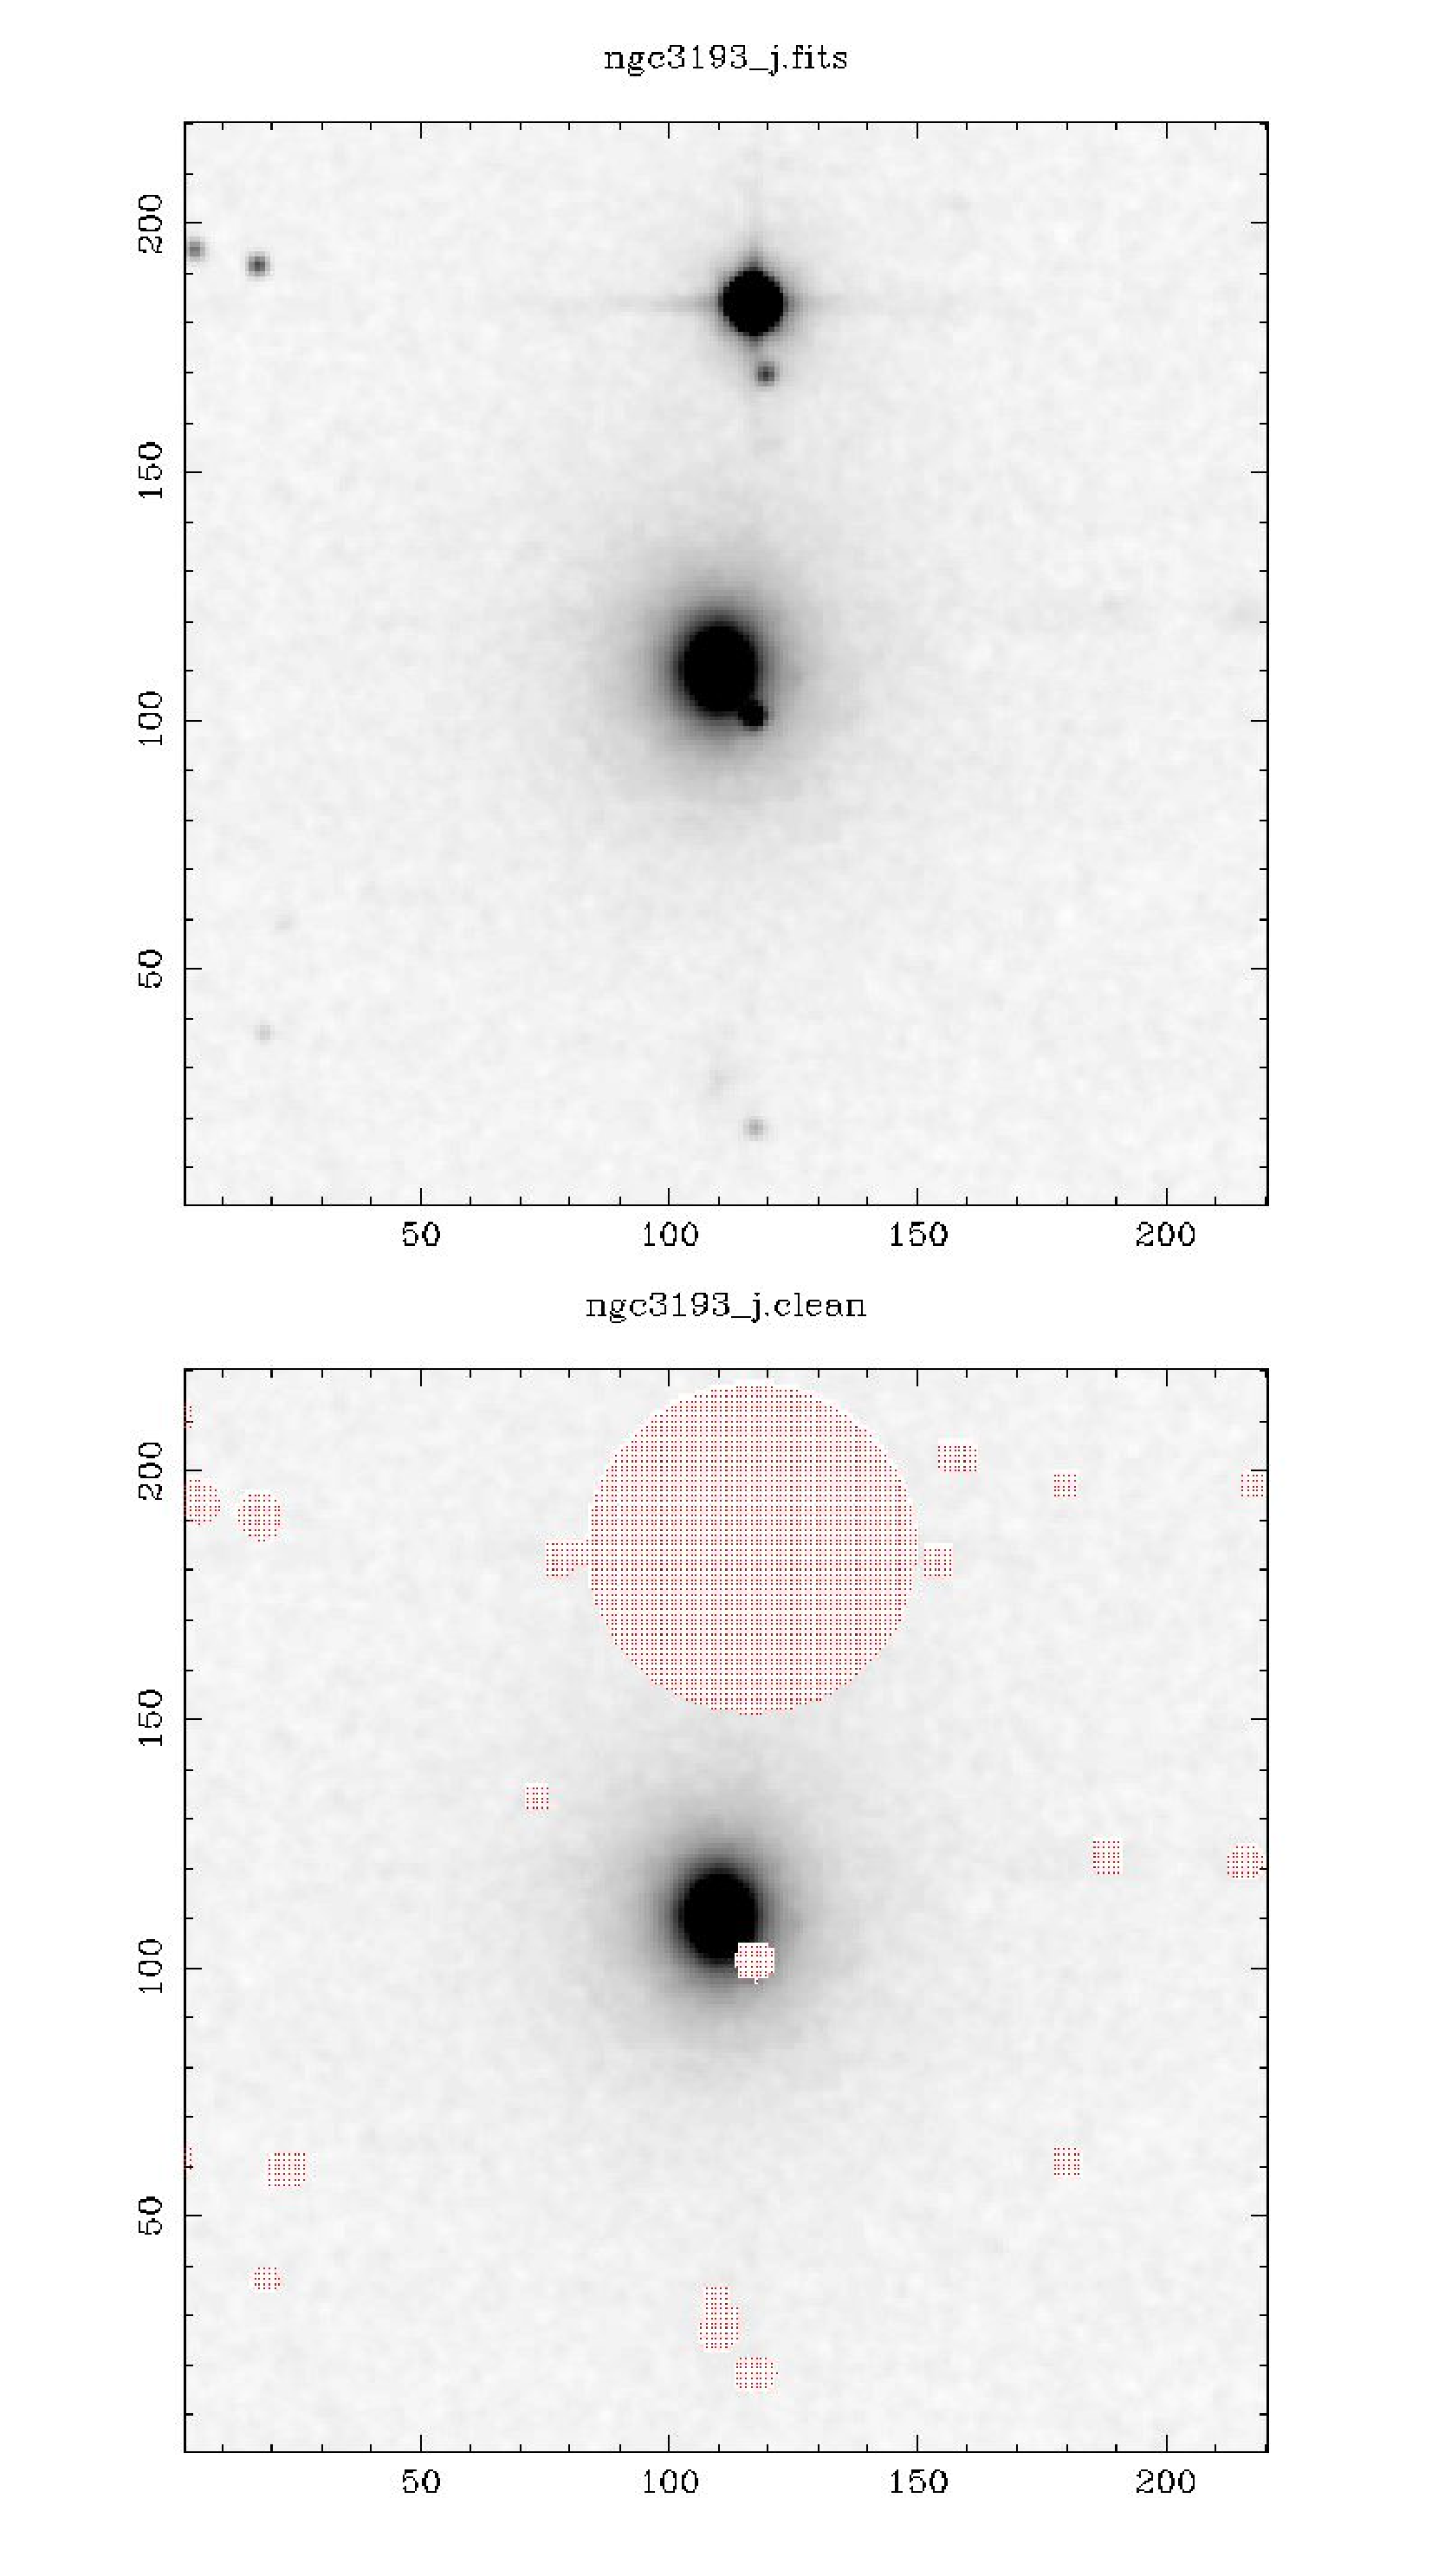
\includegraphics[scale=0.4]{ngc3193a} \caption{The raw and cleaned $J$ frames for NGC 3193, an elliptical selected
from the RSA sample (Schombert 2007). Note the proper cleaning of
contaminating stars, even a object near the galaxy core. }
\end{figure}


For a cosmetically smooth image, an efficient, but crude, sky fit
is one that simply examines the border of the frame and does an iterated
average, clipping pixels more than 4$\sigma$ from the mean. A border
sky fit is often sufficient to find the starting center of the galaxy
(for the ellipse fitting routines), clean the frame of stars/galaxies
external to the object of interest (the ellipse fitting routines will
clean along the isophotes, see below) and provide a preliminary error
estimate to the photometry. This error estimate is preliminary in
that the true limiting error in the surface (and aperture) photometry
of large galaxies is not the RMS of an isophote, but how well the
sky value is know. Once the number of pixels involved in a calculation
(be it an isophote or an aperture) becomes large (greater than 50
for typical readout noises), then the error is dominated by the precision
of the sky value.

The disadvantage to a border sky fit is the occasional inconvenient
occurrence of stars or bright galaxies on the edge of the frame. An
iterated mean calculation will remove small objects. And large objects
will be signaled with large $\sigma$'s in an iterative mean search.
In an automated procedure, more than likely, the task will have to
halt and request human intervention to find a starting sky value.

After years of experimentation, the method of choice for accurate
sky determination for extended galaxies is to evaluate sky boxes.
This is a procedure where boxes of a set sized are placed semi-randomly
(semi in the sense of avoiding stars and other galaxies) in the frame.
An algorithm calculates an iterative mean and $\sigma$ for each box.
These means (and $\sigma$'s) are then super-summed to find the value
of the sky as the mean of the means (and likewise, the error on the
sky value is the $\sigma$ on this mean).

From an analysis point of view, there are several advantages to this
technique. One is that each box exists as a measurement independent
of the other boxes. Thus, the statistical comparison of the boxes
is a real measure of the quality of the sky determination for the
frame in terms of its accuracy and any gross trends with the frame.
Another advantage is that contaminating objects are relatively easy
to avoid (visual choice of sky boxes) or to sort by the higher $\sigma$
per box. Lastly, sky boxes are the easiest method of finding regions
for sky determination outside the galaxy itself, particularly where
an irregular object may fill a majority of the data frame.

\begin{figure}
\centering 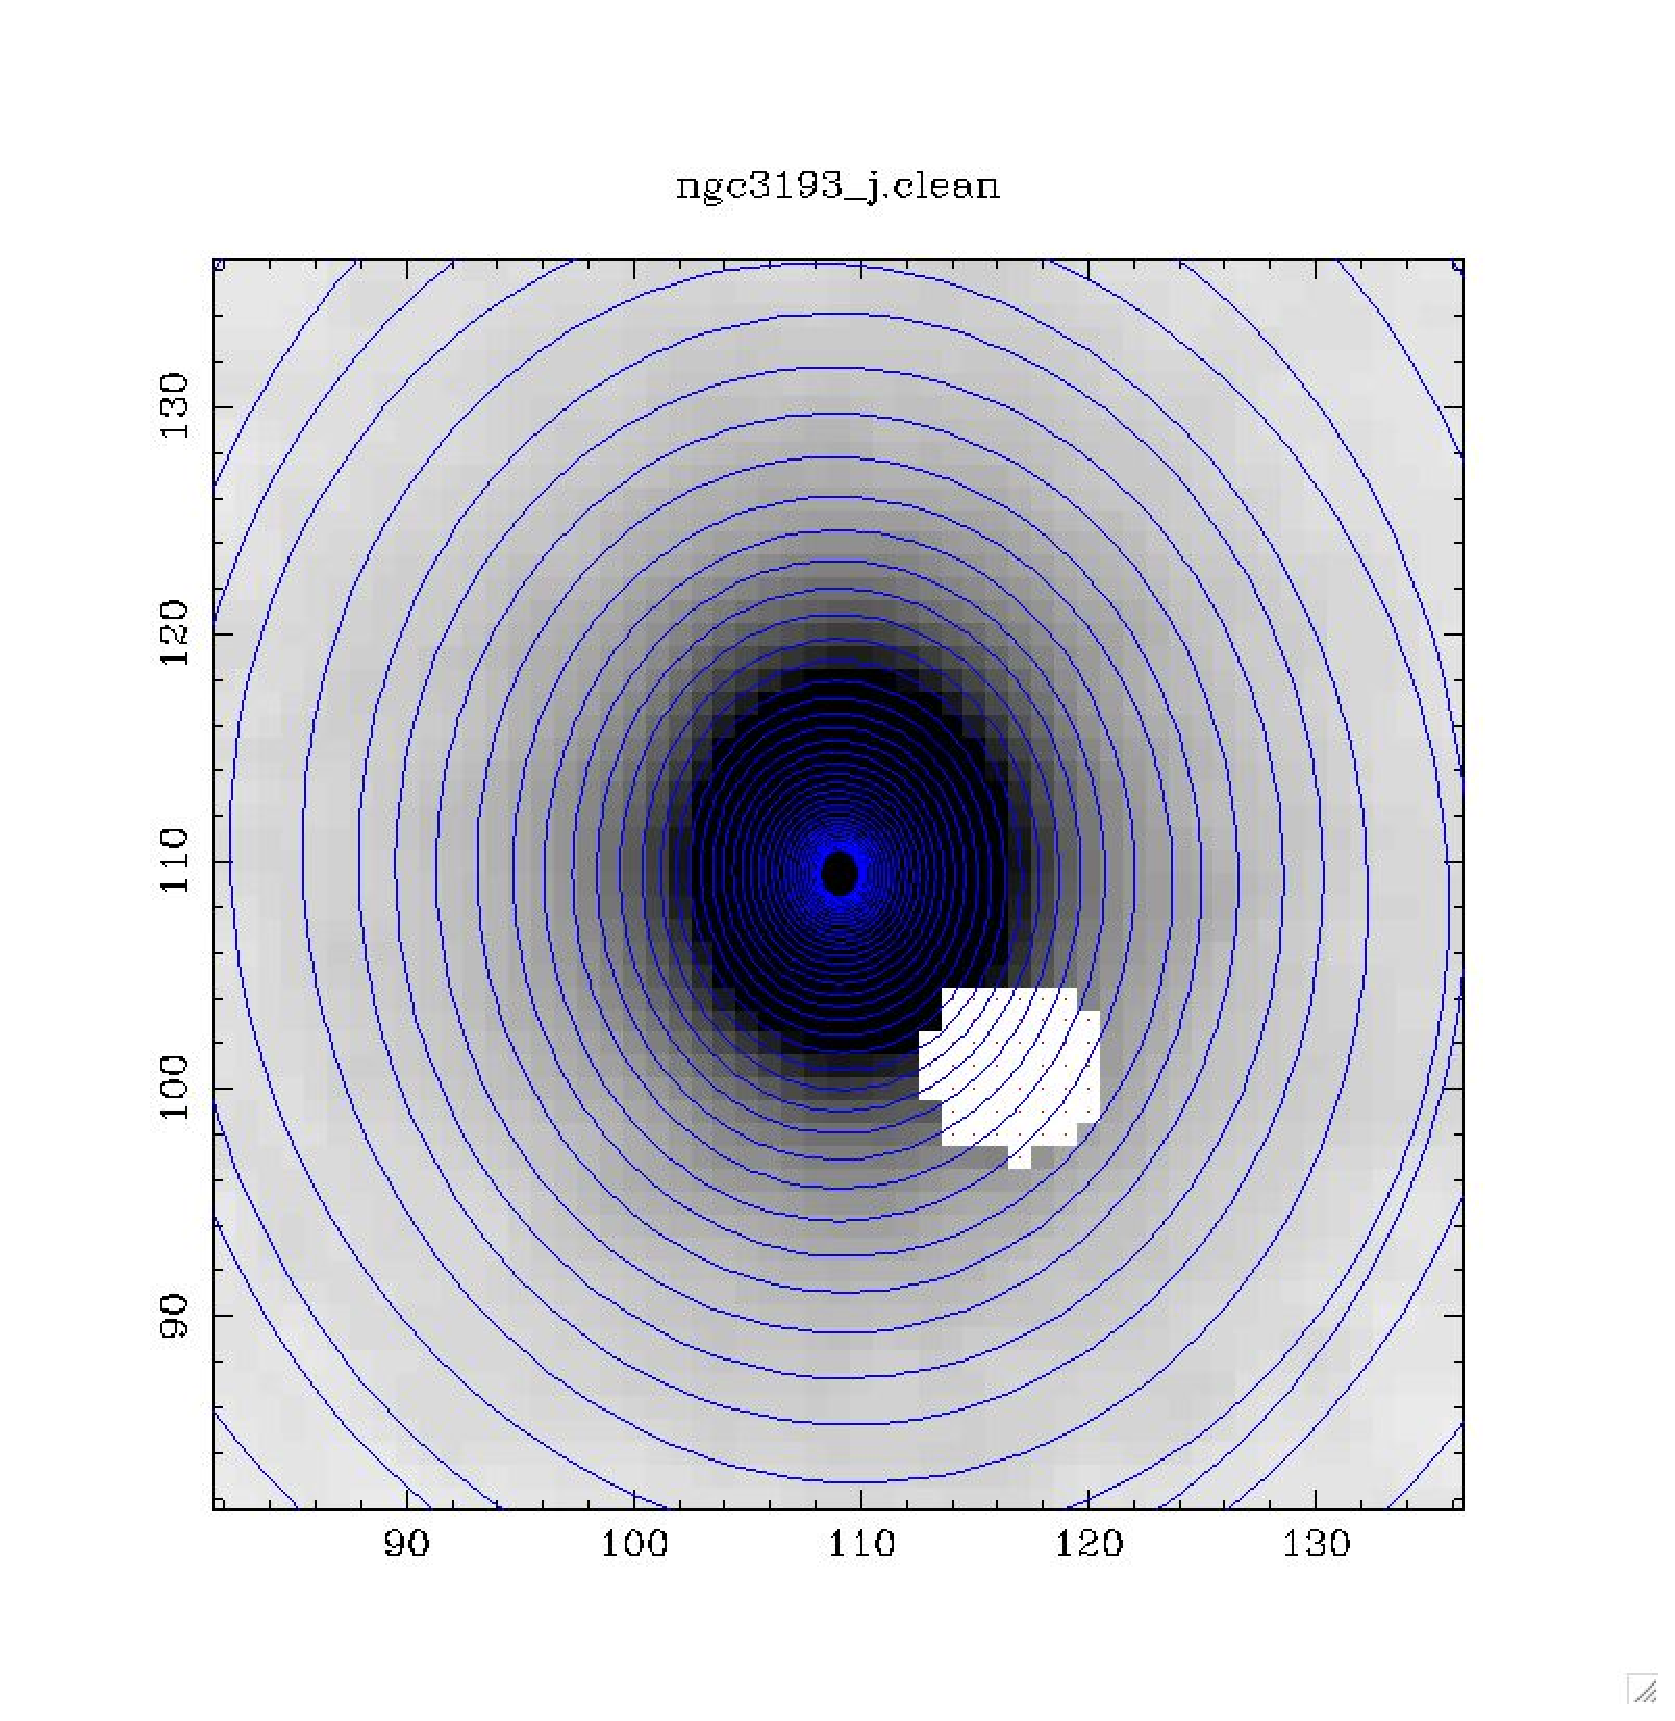
\includegraphics[scale=0.55]{ngc3193b} \caption{The resulting ellipse fits to NGC 3193's core region. While the automatic
masking of the contaminating star is not perfect, it is sufficient
to maintain a high quality fit. }
\end{figure}


The most difficult decision in sky determination by boxes is, of course,
where to place the boxes. When done visually, the user selects region
(usually with a cursor) that are free of stars and sufficiently far
away from the target galaxy to be clear of its envelope light. For
an automated process, the procedure returns for a final sky estimate
after the ellipse fitting process is completed and when all the stars/galaxies
are cleaned (set to values of not-a-number, NaN). Then, the outer
edge of the large galaxy is determined and an iterative analysis of
sky boxes outside this radius is used to determine the true sky and,
most importantly, the variation on the mean of those boxes as a measure
of how well the sky is known. This procedure is the role of \textit{sky\_box},
see the Appendix for a more detailed description of its options.


\subsection{Ellipse Fitting}

Reduction of a 2D image into a 1D run of intensity versus radius in
a galaxy assumes some shape to the isophote. Very early work on galaxies
used circles since the data was obtained through circular apertures
in photoelectric photometers. For early type galaxies, the ellipse
is the shape that most closely follows the shape of the isophotes.
This would confirm that the luminosity being traced by an isophote
is due to stellar mass, which follow elliptical orbits (Kepler's 1st
law). As one moves to along the Hubble sequence to later type galaxies,
the approximation of an ellipse to the isophotes begins to break down
due to recent star formation producing enhancements in luminosity
density at semi-random positions. However, no consistent shape describes
the isophotes of irregular galaxies, so an ellipse is the best shape,
to first order, and provides a common baseline for comparison to more
regular galaxies.

\begin{figure}
\centering 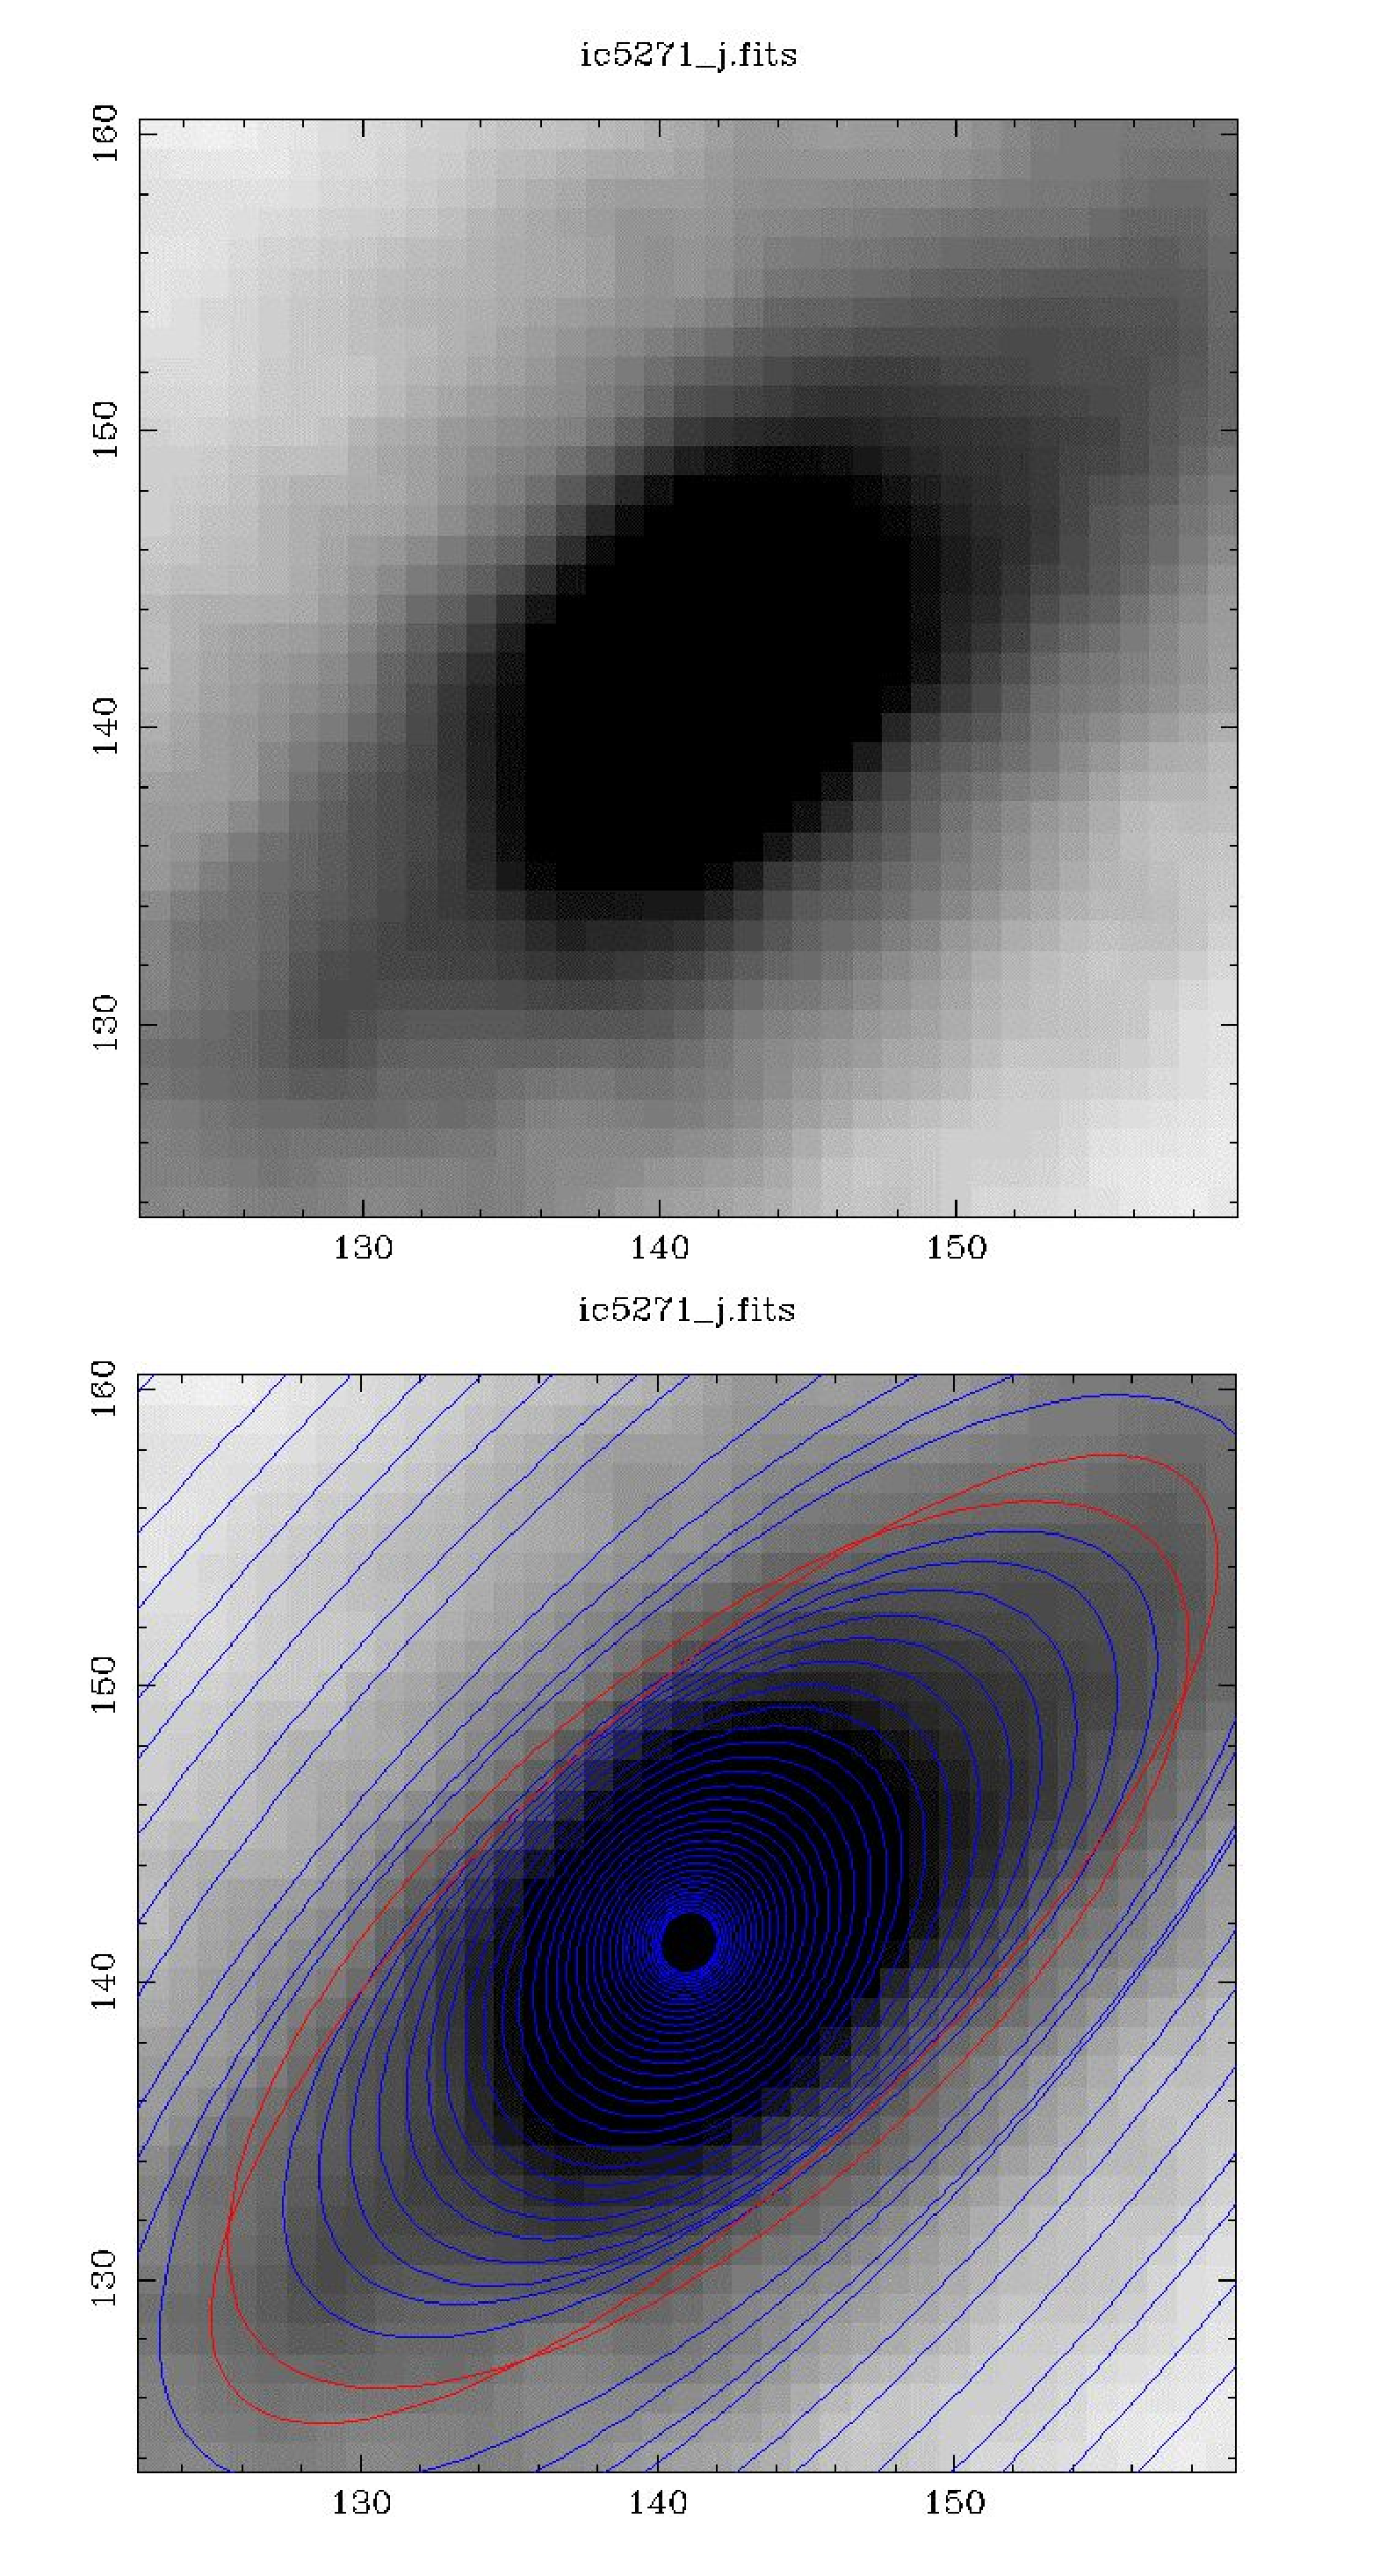
\includegraphics[scale=0.4]{ic5271} \caption{A high contrast zoom-in of the 2MASS $J$ image of IC 5271, a Sb(rs)
galaxy selected from the RSA catalog. Typical of the isophotes for
a disk/bulge galaxy, there is a cross over point as one transitions
from a more spherical bulge to a flattened disk. While this is flagged
by the reduction software, it is astrophysically real and signals
the lens morphology often seen in surface brightness profiles of disk
galaxies. }
\end{figure}


Fitting a best ellipse to a set intensity values in a 2D image is
a relatively straight forward technique that has been pioneered by
Cawson \etal (1987) and refined by Jedrzejewski (1987) (see also
an excellent review by Jensen \& Jorgensen 1999). The core routine
from these techniques (PROF) was eventually adopted by STSDAS IRAF
(i.e. ELLIPSE). The primary fitting routine in this package follows
the same techniques (in fact, uses much of the identical FORTRAN code
from the original GASP package of Cawson) with some notable additions.

These codes start with an estimated x-y center, position angle and
eccentricity to sample the pixel data around the given ellipse. The
variation in intensity values around the ellipse can be expressed
as a Fourier series with small second order terms. Then, an iterative
least-squares procedure adjusts the ellipse parameters searching for
a best fit, i.e. minimized coefficients. There are several halting
factors, such as maximum number of iterations or minimal change in
the coefficients, which then moves the ellipse outward for another
round of iterations. Once a stopping condition is met (edge of the
frame or sufficiently small change in the isophote intensity), the
routine ends. A side benefit to above procedure is that the cos(4$\theta$)
components to each isophote fit are easily extracted, which provides
a direct measure of the geometry of the isophote (i.e. boxy versus
disk-like, Jedrzejewski 1987).

One new addition, from the original routines, is the ability to clean
(i.e. mask) pixels along an isophote. Basically, this routine first
allows a few iterations to determine a mean intensity and RMS around
the ellipse. Any pixels above (or below) a multiple of the RMS (i.e.
3$\sigma$) are set to not-a-number (NaN) and ignored by further processing.
Due to the fact that all objects, stars and galaxies, have faint wings,
a growth factor is applied to the masked regions. While this process
is efficient in early-type galaxies with well defined isophotes, it
may be incorrect in late-type galaxies with bumpy spiral arms and
HII regions. The fitting will be smoother, but the resulting photometry
will be underestimated. This process can be controlled early in the
analysis pipeline by the user with an initial guess of the galaxy's
Hubble type. Also, the erased pixels are only temporary stored until
an adequate fit is found. Once a satisfactory ellipse is encountered,
only then are the pixels masked for later ellipse fitting. The masked
data is written to disk at the end of the routine as a record of the
cleaning. The ellipse fitting is the function of \textit{efit} as
described in the Appendix.

For early-type galaxies, lacking any irregular features, the cleaning
process is highly efficient. The pipeline first identifies the galaxy
and its approximate size by moment analysis. It then cleans off stars/galaxies
outside the primary galaxy by moment identification and radius growth
for masking. Stars/galaxies inside the primary galaxy are removed
by the ellipse fitting routine. The resulting ellipses are inspected
for crossover (isophotes that crossover are assumed to be due to errors
or embedded stars/galaxies and removed by averaging nearby ellipse
isophotes, this is not true for disk galaxies). The smoothed ellipses
are used by a more robust cleaning algorithm and the whole ellipse
fitting process is repeated on the cleaned frame.

\begin{figure}
\centering 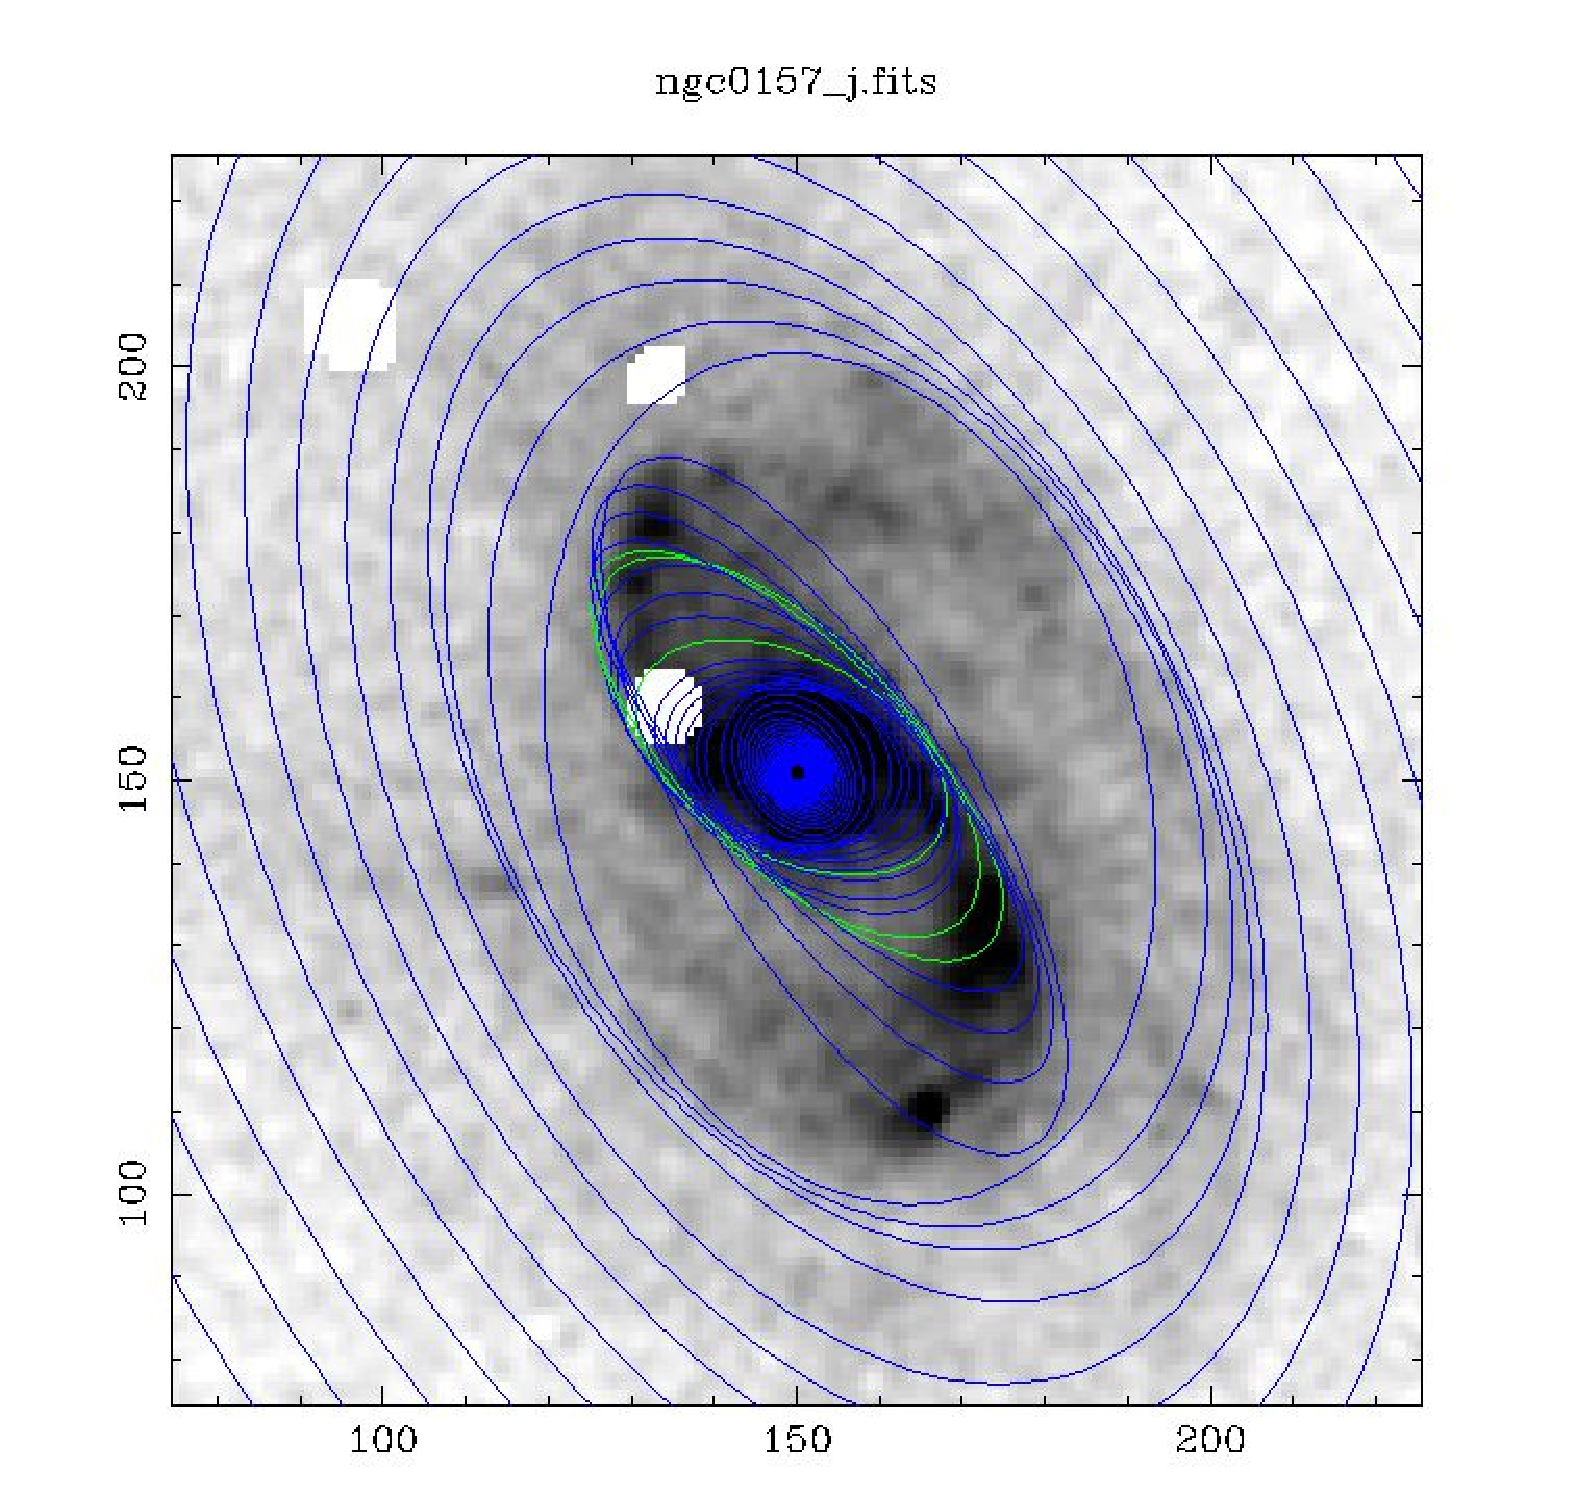
\includegraphics[scale=0.45]{ngc0157a} \caption{A high contrast zoom-in of the 2MASS $J$ image of NGC 157, a face-on
Sc(s) galaxy selected from the RSA catalog. Similar to IC 5271, there
are several crossover points in the fitted ellipses. The fitting program
does a good job of following the spiral arms in the inner regions,
then a large jump from bulge to disk region. }
\end{figure}


An example of the analysis of an elliptical is found in Figure 1,
a 2MASS $J$ image of NGC 3193. The top panel is the raw 2MASS image,
the bottom panel is the resulting cleaned image output at the end
of the reduction process. The cleaning process efficiently removed
all the stars on the frame, including the brighter object on the northern
edge of the frame and its diffraction spikes. The star closest to
the galaxy core is a problem in two arenas. The first is in the calculation
of ellipse, as the inner star would drag the calculated moments off
center. The isophote erasing routine has handled this as can be seen
in Figure 2, where the fitting ellipses are shown and are not deflected
by the erased star. Second, is that calculated total magnitudes would
either be over estimated (if the star is not masked) or under estimated
(if the star is masked and the galaxy light from those pixels is not
replaced). This problem will be discussed in \S 2.6.

As one goes towards later type galaxies, there is an increase in the
non-elliptical nature to their isophotes and an increase in luminosity
density enhancements (HII regions, stellar clusters, spiral features)
which are legitimate components to the galaxy's light distribution
and should not be cleaned. The user can specify the galaxy type and
the cleaning restrictions will be tightened (only to stellar objects
and at a higher cleaning threshold) plus the restrictions on overlapping
ellipses is loosened (e.g. the transition from a round bulge to a
flat disk). Most importantly, while some galaxy features are cleaned
for the sake of a harmonious ellipse fit, those pixels need to be
filled for later aperture photometry.

\begin{figure}
\centering 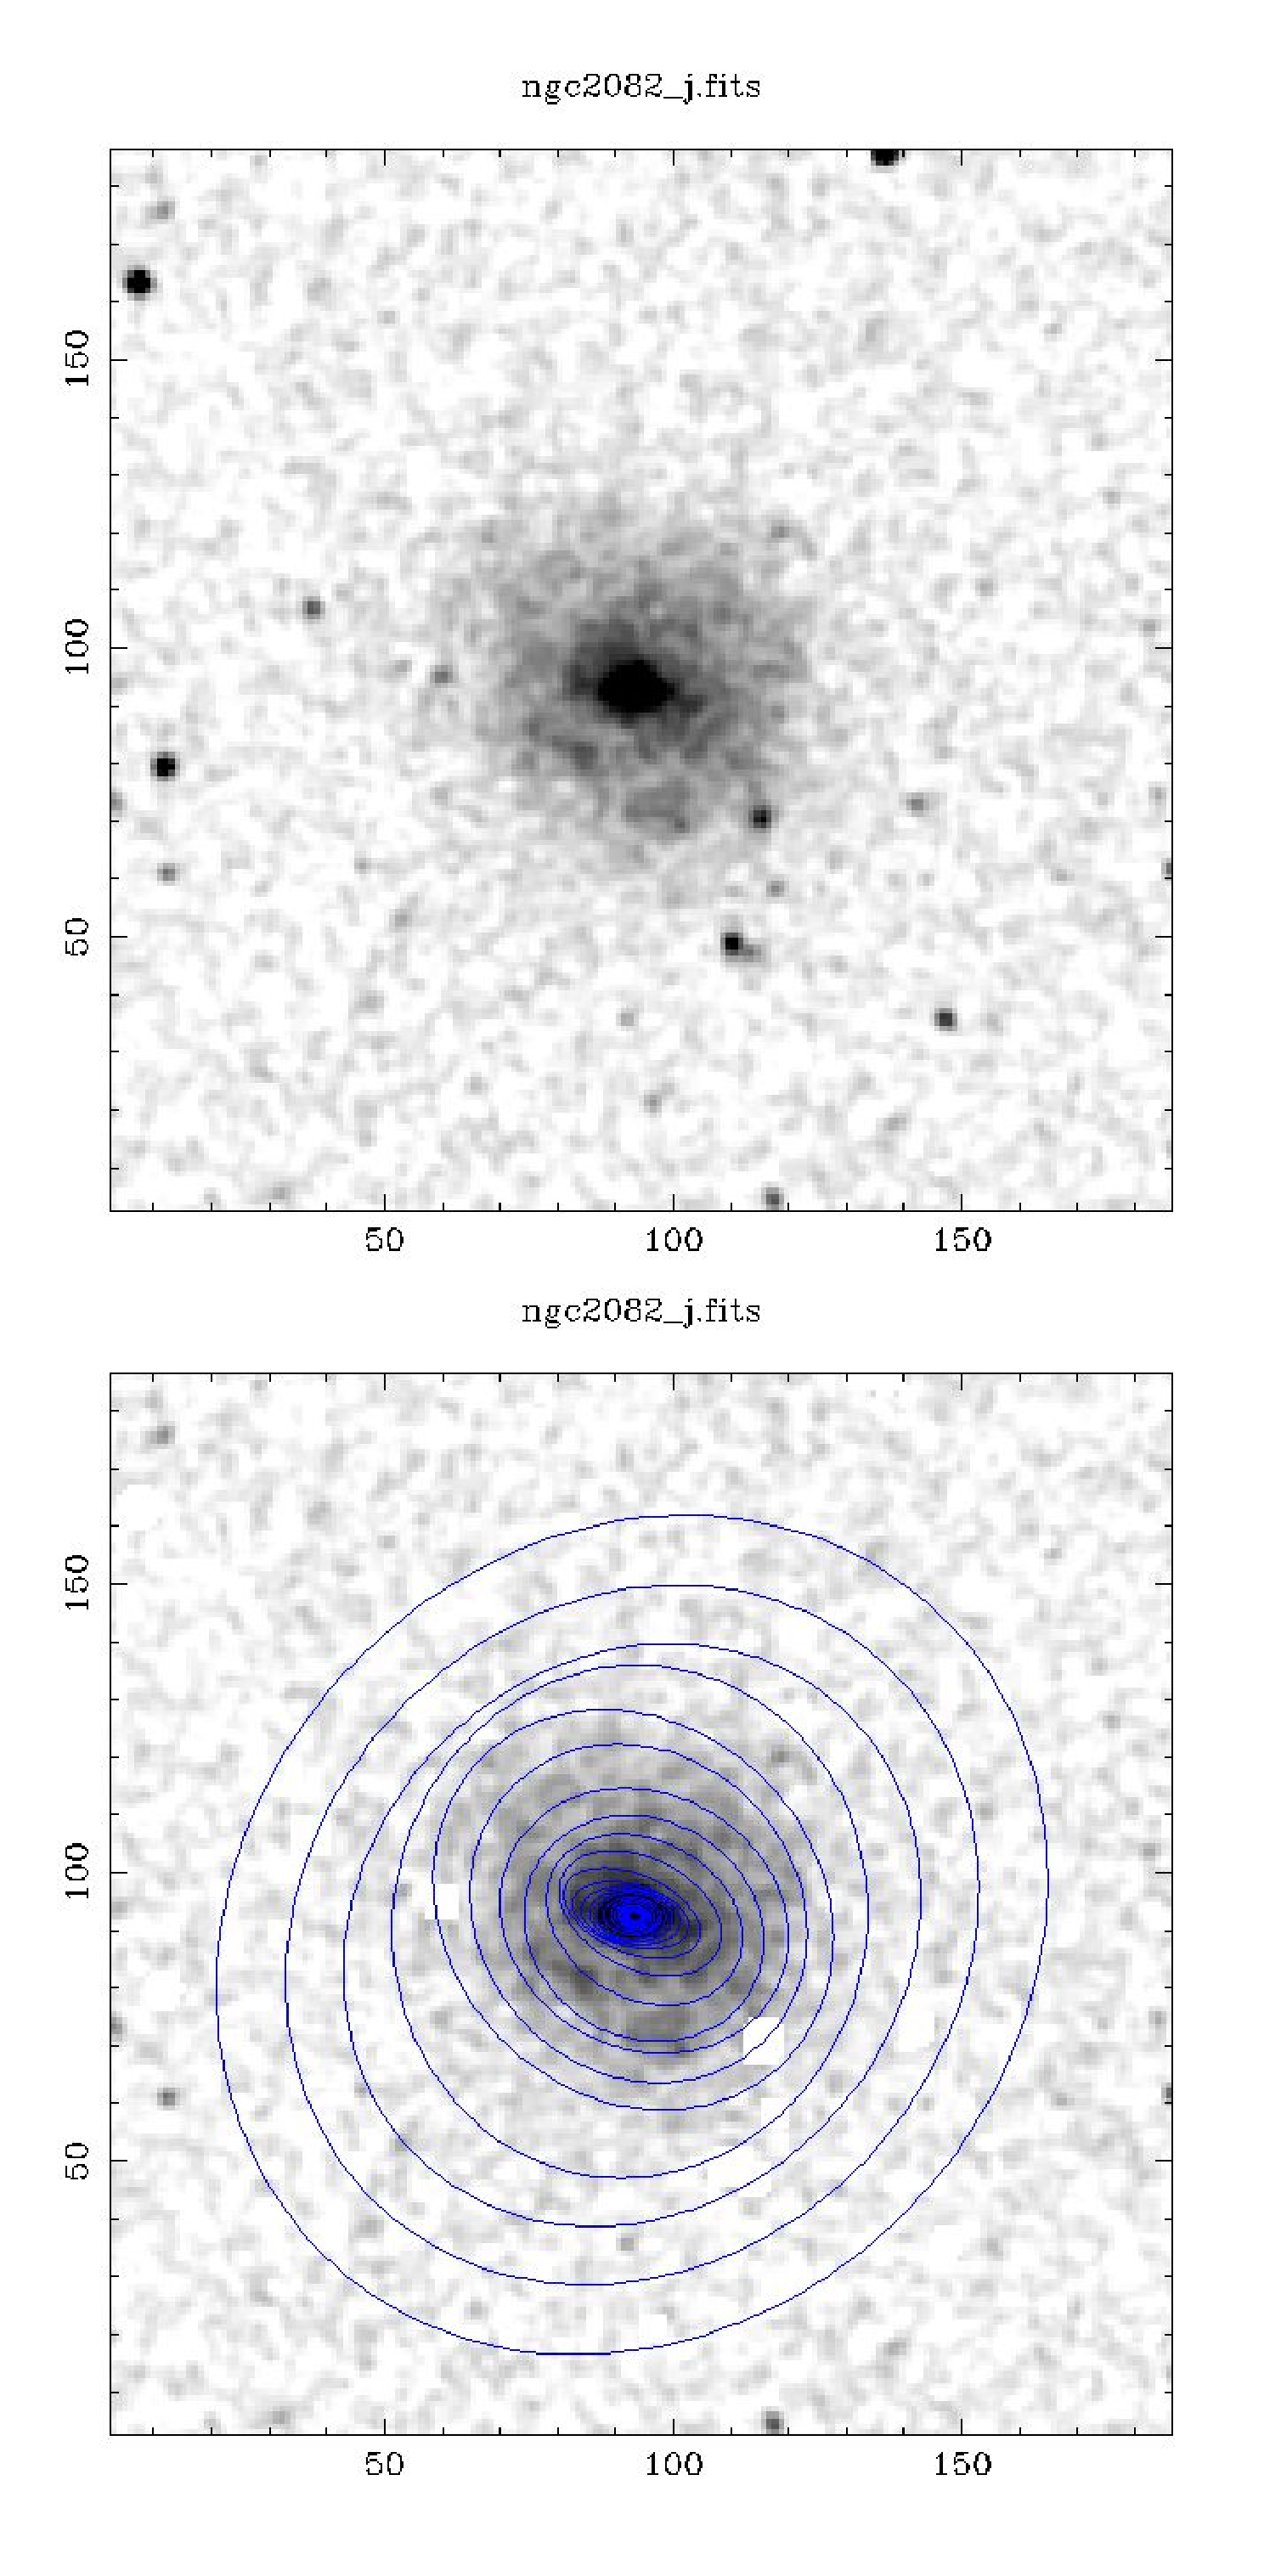
\includegraphics[scale=0.4]{ngc2082} \caption{A high contrast subimage of the 2MASS $J$ image of NGC 2082, a LSB
disk galaxy. Note, that the ellipse fitting routine expanded the annulus
size to increase the S/N. }
\end{figure}


An example of this behavior can be found in Figure 3, the $J$ image
of IC 5271. The red ellipses indicate isophote fits that crossover.
While flagged as an error, this is in fact the real behavior of the
isophotes as one transitions from bulge to disk. The resulting intensities
are probably overestimated due to the crossover effect, but this error
will be minor compared to the errors that would result from an off-center
or overly round ellipse.

The quality of the fitting procedure can be judged by the behavior
of the ellipse parameters such as eccentricity, position angle and
center. If there are large jumps in any of the parameters that determine
shape, then this may signal a feature in the galaxy that needs to
be cleaned (a buried star for example). Slightly less abrupt changes
may signal an astrophysically interesting features, such as a bar
or lens morphology. Under the assumption that the isophotes of a typical
galaxy are a smooth function with radius, the ellipse fitting algorithm
checks for ellipse parameters that indicate a crossing of the isophotal
lines. These ellipses are smoothed and flagged (the mean of the inner
and outer ellipse parameters is used). In certain scenarios, crossing
isophotes are to be expected, for example the transition region from
a bulge to a disk (see Figure 2), and the smoothing criteria is relaxed.
This is the function of $prf\_smooth$ as described in the Appendix.

\begin{figure}
\centering 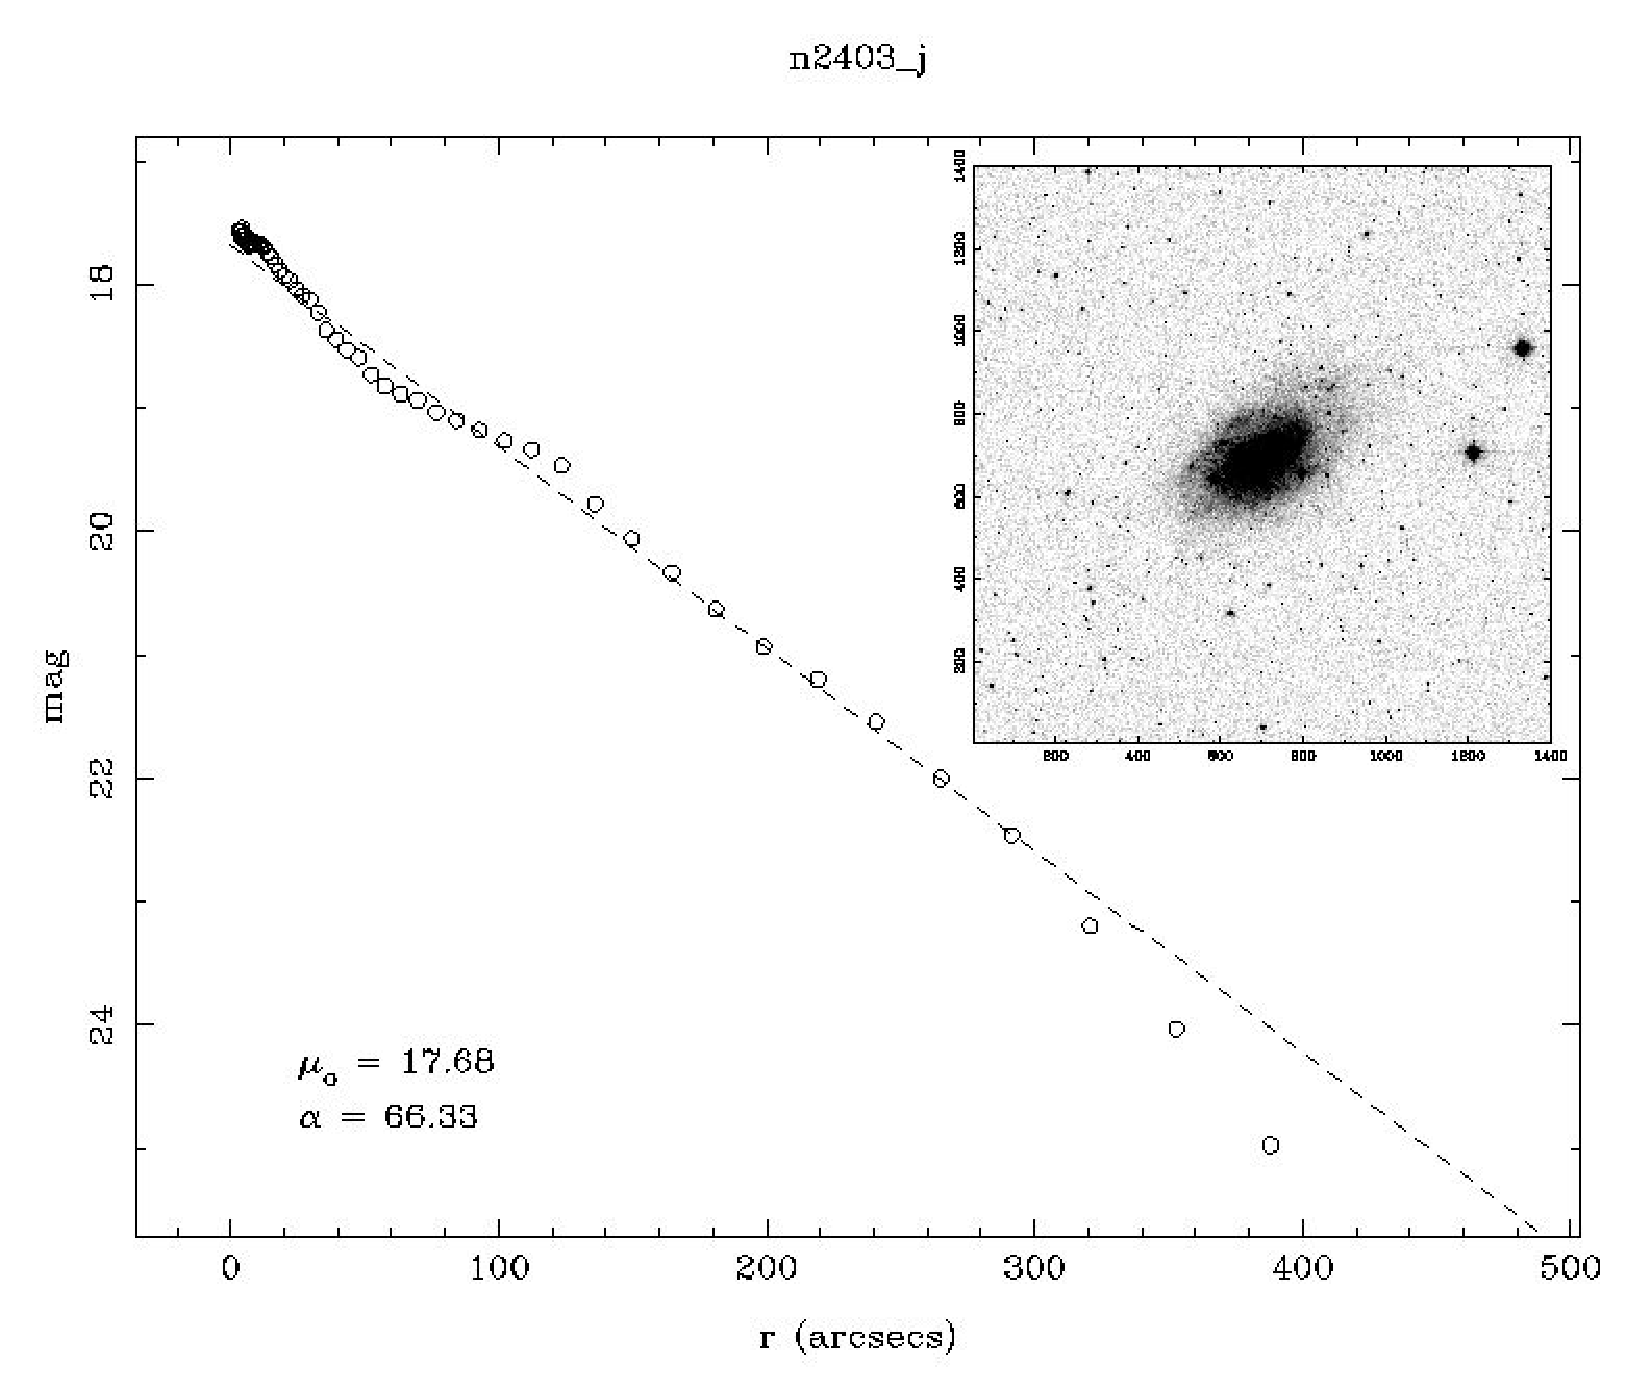
\includegraphics[scale=0.45]{ngc2403_sfb} \caption{A final surface brightness profile for NGC 2403, an Sc(s) galaxy.
The dotted line is a bi-weighted linear fit along with the resulting
fit parameters. }
\end{figure}


An example of $prf\_smooth$'s corrections can be seen in Figure 4,
the $J$ image of NGC 157. Several interior ellipses display erratic
behavior, but $prf\_smooth$ took the mean average of nearby ellipses
(in green) to produce a more rational fit. The resulting intensities
were also more stable, although the RMS is going to be highly than
the typical isophotes found in an elliptical.

An example of a LSB galaxy fit is found in Figure 5. The ellipse fitting
routine, recognizing that the target is low in contrast with respect
to sky, widened the annulus for collecting pixel values. This increases
the S/N at some loss of spatial resolution. Since resolution is usually
not important in a galaxy's halo region, this is an acceptable trade
off. LSB galaxies are susceptible to fitting instability, the fitting
routines are tightened against rapid changes in eccentricity and centering
to prevent this behavior.

LSB galaxies also demonstrate a key point in determining errors from
surface photometry. There are two sources of error per isophote, the
RMS around the ellipse and the error in the sky value. The RMS value
is a simple calculation using the difference between the mean and
the individual pixel values. This RMS then reflects into an observable
error as the $\sqrt{N}$. However, as the isophote intensity approaches
the sky value, the number of pixels increases and the error due to
RMS becomes an artificially low value. In fact, at low intensities,
the knowledge of the sky value dominates and the error in the isophote
is reflected by the sky error (preferably as given by the $\sigma$
on the means of a large number of sky boxes).


\subsection{Surface Photometry}

With a file of isophotal intensities versus radius in hand, it is
a simple step to producing a surface brightness profile for the galaxy.
There are a few tools are in the package to examine the quality of
the ellipse fitting (e.g. $prf\_edit$, an interactive comparison
of the image and the ellipses). At the very least, a quick visual
inspection of the ellipses seems required as a bad mismatch leads
to strongly biased results (see cautionary tale in \S 4). A user
can either step through a directory of data files (e.g. using the
$probe$ tool) or a user can automatically produce a group of GIF
images with a corresponding HTML page, then use a browser to skim
through a large number of files. Calibration from image data numbers
(DN) to fluxes (or magnitudes) is usually obtained through standard
stars with corrections for airmass and instrumental absorption. If
these values are in the FITS headers, then they are automatically
added to the object's XML file. Additional corrections for galactic
absorption, k-corrections and surface brightness dimming are well
documented in the literature and can be assigned automatically by
grabbing XML data from NED. A chosen cosmology converts radius in
pixel units into astrophysically meaningful values of kiloparsecs.
A Python command line script ($cosmo$) based on Ned Wright's cosmology
calculator is included in the package All these values can be added
to the XML file for automatic incorporation to the analysis programs.
If they don't exists, then instrumental mags will be used, which can
easily be converted to real units later on.

\begin{figure}
\centering 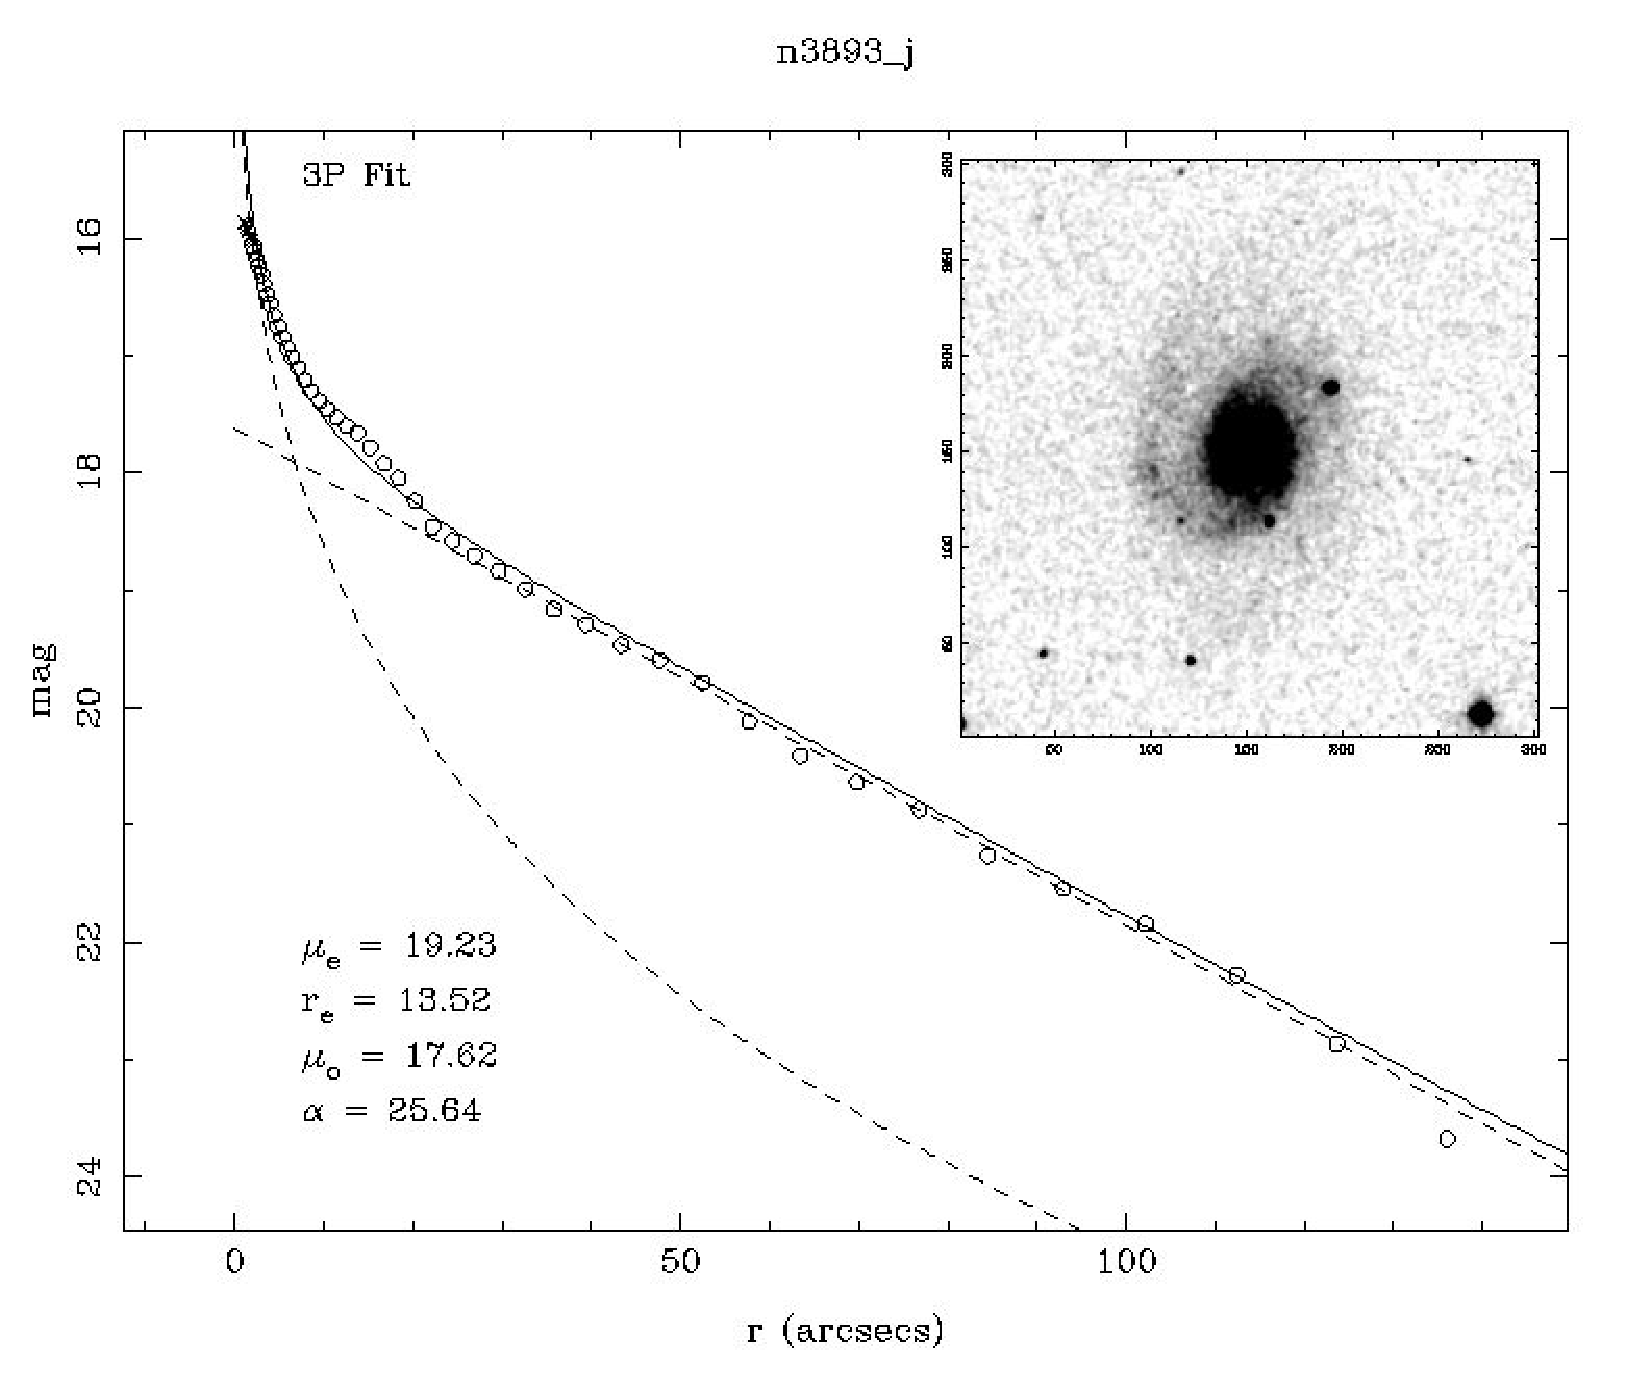
\includegraphics[scale=0.45]{ngc3893_sfb} \caption{A final surface photometry profile for NGC 3893, an Sc(s) galaxy.
The dotted lines are exponential and r$^{1/4}$ fits to disk and bulge.
The solid line is the addition of the two curves. }
\end{figure}


Analysis of a 1D surface brightness profile (the job for the $bdd$
tool) depends on the scientific goals of the user. For example, early-type
galaxies are typically fit to a de Vaucouleurs r$^{1/4}$ curve to
extract a scale length (effective radius) and characteristic surface
brightness (effective surface brightness). Irregular and dwarf galaxies
are well fit by exponential profiles which provide a disk scale length
and central surface brightness. Disk galaxies can be fit with a combination
of bulge and disk fits, to extract B/D ratios and disk scale lengths.

Due to this combination of $r^{1/4}$ and exponential curves for large
bulge spirals, it is computationally impossible to correctly determine
which function, or combination of functions, best fits a particular
galaxy's profile. In the past, one would examine the 2D image of the
galaxy and obvious disk-like galaxies would be fit to $r^{1/4}$ plus
exponential. Objects with elliptical appearance were fit to a strict
$r^{1/4}$ shape. This produces a problem for large bulge S0's which
are difficult to detect visually unless nearly edge-on.

The simplest solution to this problem, using only the 1D surface photometry,
is to examine the profiles in a plot of mag arcsecs$^{2}$ versus
linear radius. With this plot, exponential disks appear as straight
lines, see Figure 6 as an example of a pure disk in NGC 2403. Bulge
plus disk components are also straight forward in this mag/linear
radius space, see Figure 7 a good example of a bulge plus disk fit
in NGC 3983. If a profile displays too much curvature, with no clear
linear disk portion, then it is a good candidate for a pure $r^{1/4}$
fit (see Figure 8, NGC 3193). This option is easily checked by plotting
the profile in mag arcsecs$^{2}$ versus r$^{1/4}$ space as shown
in Figure 8. Most r$^{1/4}$ profiles only have a linear region in
the middle of the surface brightness profile, typically with a flattened
core and fall-off at large radii (see Schombert 1987).

\begin{figure}
\centering 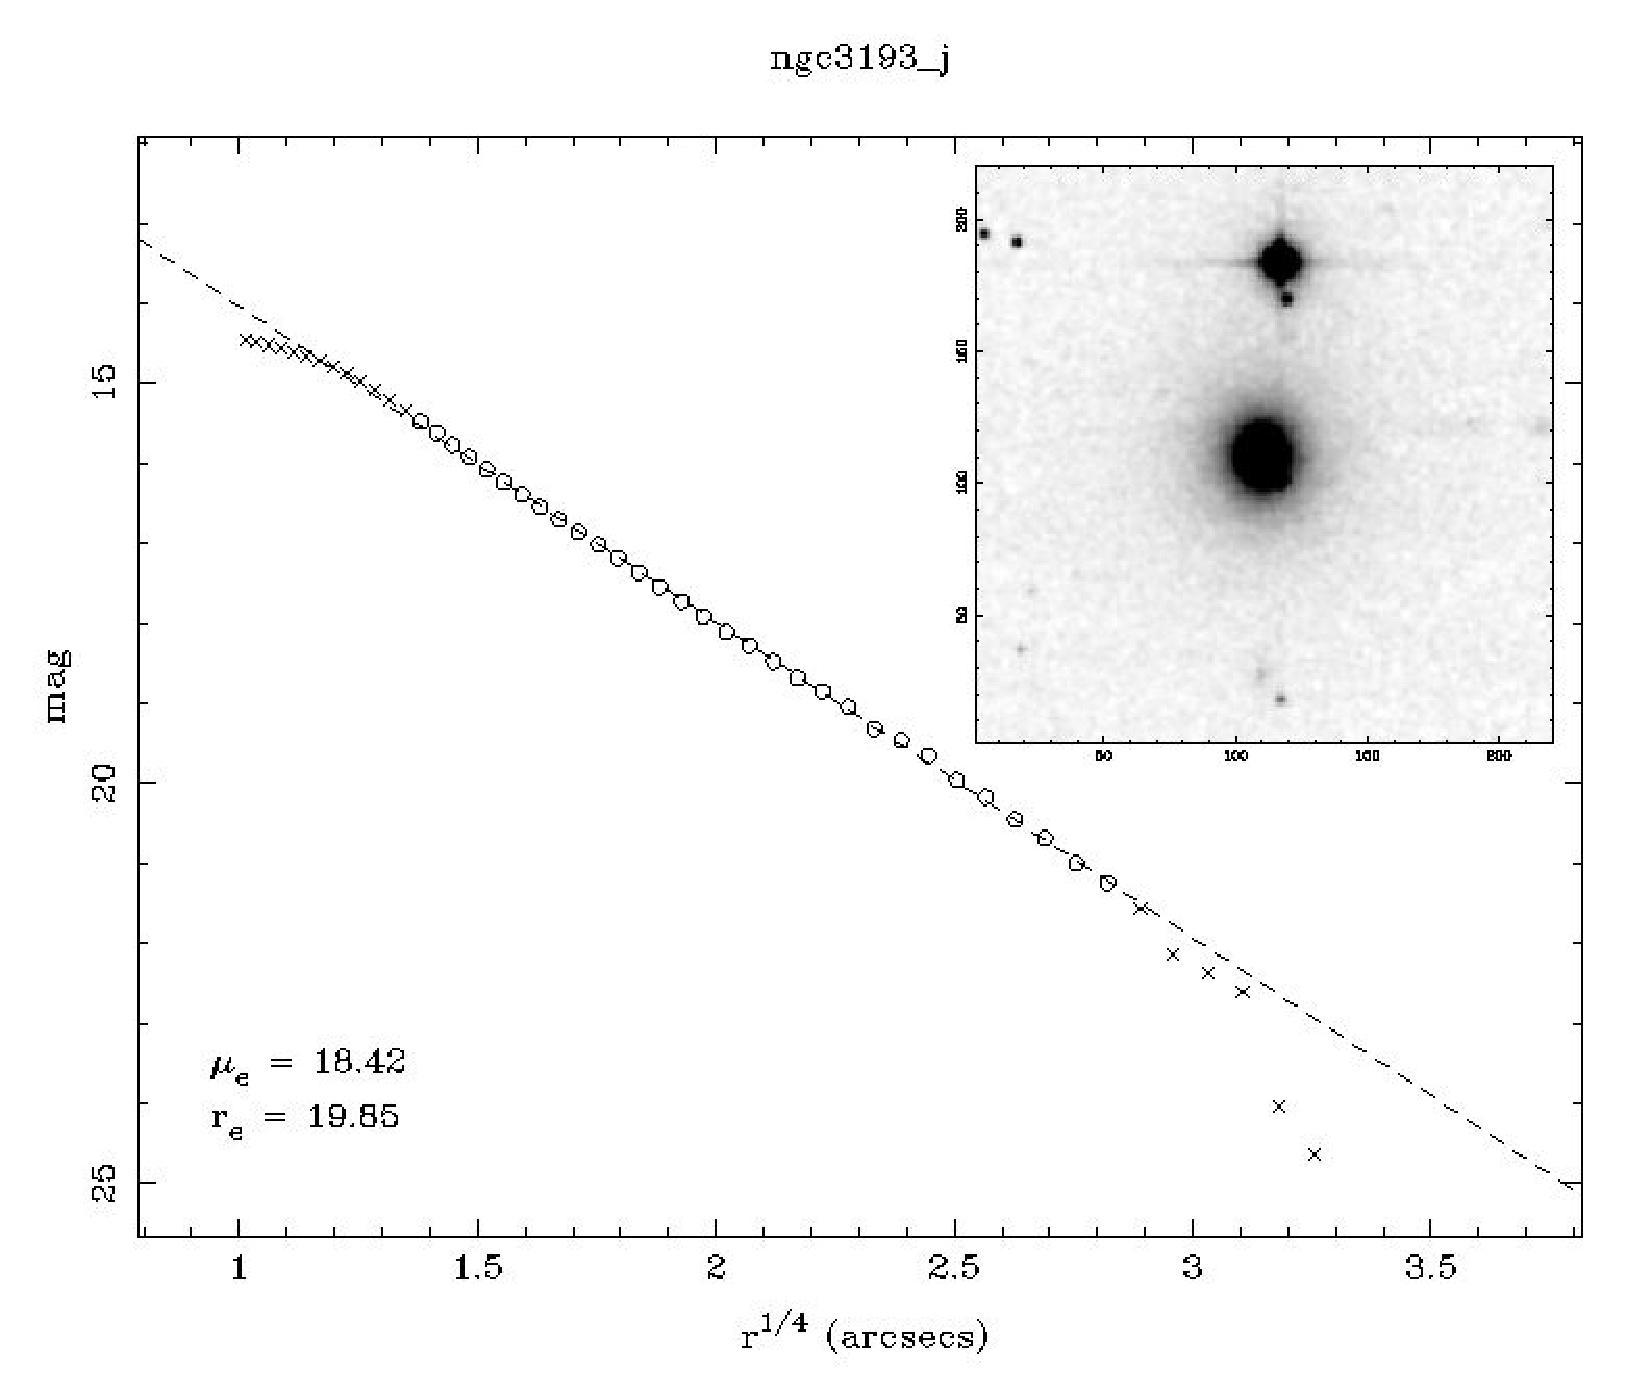
\includegraphics[scale=0.45]{ngc3193_sfb} \caption{A final surface photometry profile for the elliptical NGC 3193. A
pure r$^{1/4}$ fit is shown. }
\end{figure}


The Sersic function is also popular for fitting surface brightness
profiles (Graham \& Driver 2005), although not currently supported
by this package, any fitting function is easy to add to the reduction
routines as the core search routine is a grid search $\chi^{2}$ minimization
technique. However, there are issues with surface photometric data
where the inner regions have the highest S/N but the outer regions
better define a galaxy's structure (Schombert \& Bothun 1987). With
user guidance, this grid search works well for any user defined function.
Also, since there are a sufficient number of packages for fitting
1D data in the community, this package only provides a simple graphic
plotting function. More sophisticated analysis needs guidance by the
user, but this package provides the framework for just such additions.


\subsection{Aperture Photometry}

Often the scientific goal of a galaxy project is to extract a total
luminosity for the system (and colors for multiple filters). For small
galaxies, a metric aperture or isophotal magnitude is suitable for
comparison to other samples (certainly the dominate source of error
will not be the aperture size). However, for galaxies with large angular
size (i.e. many pixels), their very size makes total luminosity determination
problematic.

\begin{figure}
\centering 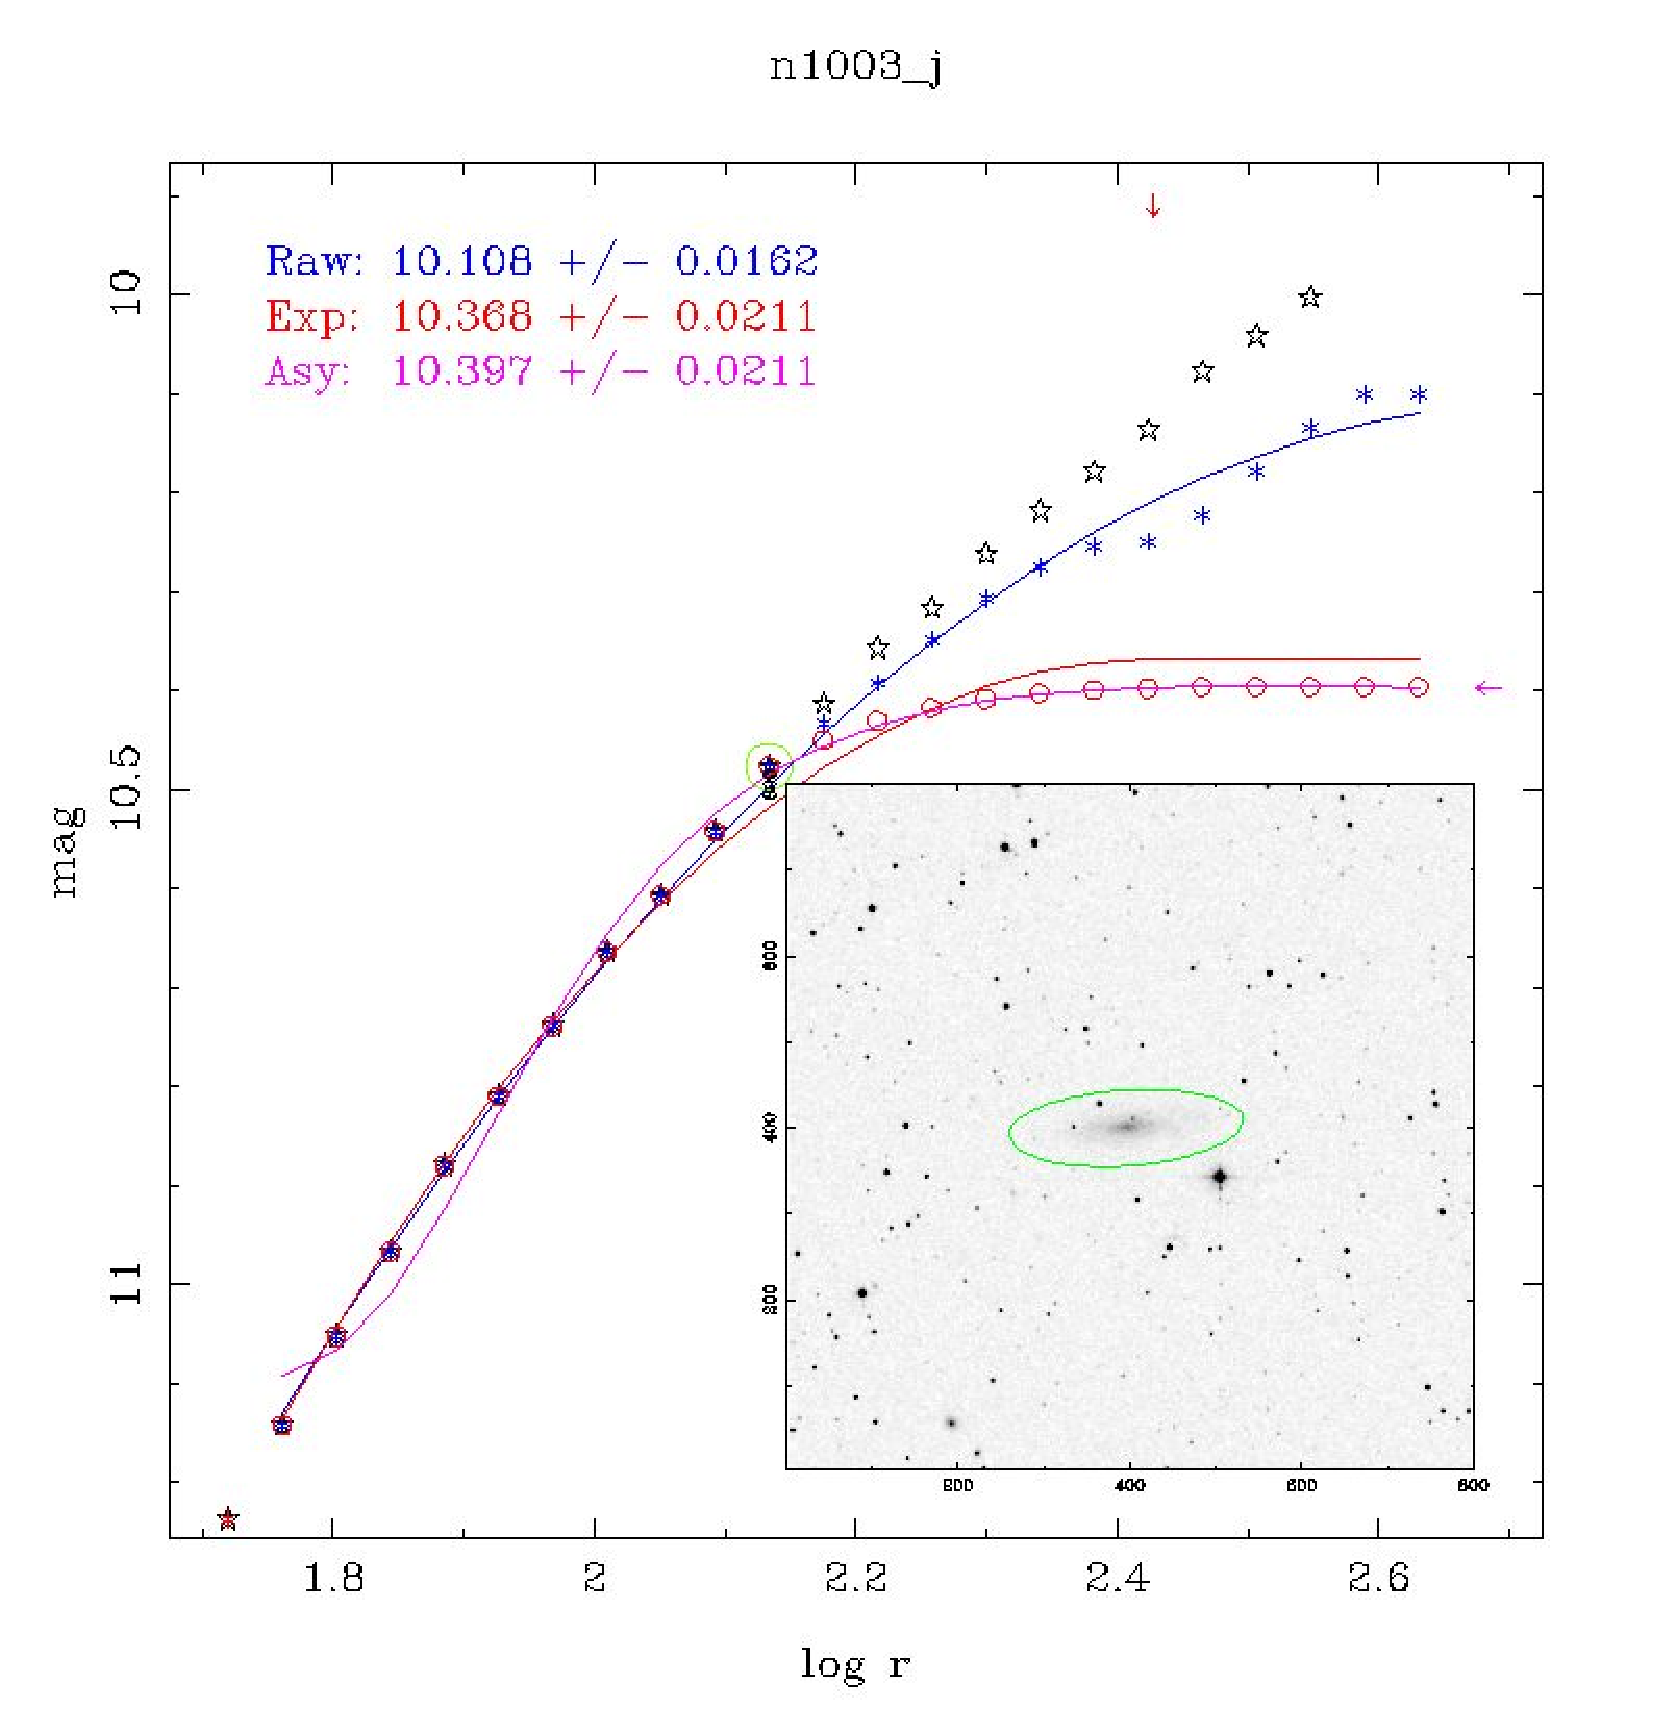
\includegraphics[scale=0.45]{n1003_asym} \caption{Elliptical aperture photometry of LSB galaxy, NGC 1003. Starred data
is the raw intensities, asterisks are apertures determined from ellipse
fitted isophotes, circles are interpolation from the surface brightness
fits. Blue and orange lines are 2nd order polynomial fits, the pink
line is a fit using rational functions. }
\end{figure}


Natively, one would think that a glut of pixels would make the problem
of determining a galaxies luminosity easier, not more difficult. However,
the problem here arises with the question of where does the galaxy
stop? Or, even if you guess an outer radius, does your data contain
all the galaxy's light? The solution proposed by de Vaucouleurs' decades
ago is to use a curve of growth (de Vaucouleurs 1977). Almost all
galaxies follow a particular luminosity distribution such that the
total light of a galaxy can be estimated by using a standard growth
curve to estimate the amount of light outside your largest aperture.
For a vast majority of galaxies, selecting either an exponential or
r$^{1/4}$ curve of growth is sufficient to adequately describe their
total luminosities (Burstein \etal 1987). However, for modern large
scale CCD imaging, the entire galaxy can easily fit onto a single
frame and there is no need for a curve of growth as all the data exists
in the frame.

With adequate S/N, it would seem to be a simple task to place a large
aperture around the galaxy and sum the total amount of light (minus
the sky contribution). However, in practice, a galaxy's luminosity
distribution decreases as one goes to larger radii, when means the
sky contribution (and, thus, error) increases. In most cases, larger
and larger apertures simply introduce more sky noise (plus faint stars
and other galaxies). And, to further complicate matters, the breakover
point in the optical and near-IR, where the galaxy light is stronger
than the sky contribution will not contain a majority of the galaxy's
light. So the choice of a safe, inner radius will underestimate the
total light.

The procedure selected in this package, after some numerical experimentation,
is to plot the aperture luminosity as a function of radius and attempt
to determine a solution to an asymptotic limit of the galaxy's light.
This procedure begins by summing the pixel intensities inside the
various ellipses determined by $efit$. For small radii, a partial
pixel algorithm is used to determine aperture luminosity (using the
surveyors technique to determine each pixel's contribution to the
aperture). At larger radii, a simply sum of the pixels, and the number
used, is output. In addition, the intensity of the annulus based on
the ellipse isophote and one based on the fit to the surface photometric
profile are also outputted at these radii (see below).

Note that a correct aperture luminosity calculation requires that
both a ellipse fit and a 1D fit to the resulting surface photometry
has be made. The ellipse fit information is required as these ellipses
will define the apertures, and masked pixels are filled with intensities
given by the closest ellipse. A surface photometric fit allows the
aperture routine to use a simple fit to the outer regions as a quick
method to converge the curve of growth.

Once the aperture luminosities are calculated, there are two additional
challenges to this procedure. The first is that an asymptotic fit
is a difficult calculation to make as the smallest errors at large
radii reflect into large errors for the fit. Two possible solutions
are used to solve this dilemma. The first solution is to fit a 2nd
or 3rd order polynomial to the outer radii in a luminosity versus
radius plot. Most importantly for this fit, the error assigned the
outer data points is the error on the knowledge of the sky, i.e. the
RMS of the mean of the sky boxes. This is the dominant source of error
in large apertures and the use of this error value results in a fast
convergence for the asymptotic fit. The resulting values from the
fit will be the total magnitude and total isophotal size, determined
from the point where the fit has a slope of zero. A second solution
is to use an obscure technique involving rational functions. A rational
function is the ratio of two polynomial functions of the form

\[
f(x)=\frac{{a_{n}x^{n}+a_{n-1}x^{n-1}+...+a_{2}x^{2}+a_{1}x+a_{0}}}{{b_{m}x^{m}+b_{m-1}x^{m-1}+...+b_{2}x^{2}+b_{1}x+1}}
\]


\noindent where $n$ and $m$ are the degree of the function. Rational
functions have a wide range in shape and have better interpolating
properties than polynomial functions, particularly suited for fits
to data where an asymptotic behavior is expected. A disadvantage is
that rational functions are non-linear and, when unconstrained, produce
vertical asymptotes due to roots in the denominator polynomial. A
small amount of experimentation found that the best rational function
for aperture luminosities is the quadratic/quadratic form, meaning
a degree of 2 in the numerator and denominator. This is the simplest
rational function and has the advantage that the asymptotic magnitude
is simply $a_{2}/b_{2}$, although is best evaluated at some radii
in the halo of the galaxy under study.

Usually the aperture luminosity values will not converge at the outer
edges of a galaxy. This is the second challenge to aperture photometry,
correct determination of the luminosity due to the faint galaxy halo.
This is where the surface photometry profile comes in handy. Contained
in that data is the relationship between isophotal luminosity and
radius, using all the pixels around the galaxy. This is often a more
accurate number than attempting to determine the integrated luminosity
in an annulus at the same radius. This information can be used to
constraint the curve of growth in two ways. One, we can use the actual
surface brightness intensities and convert them to a luminosity for
each annulus at large radii. Then, this value can be compared to the
aperture value and a user (or script) can flag where the two begin
to radically deviate. Often even the isophotal intensities will vary
at large radii and, thus, a second, more stable method is to make
a linear fit of an exponential, r$^{1/4}$ or combined function to
the outer radii and interpolate/extrapolate that fit to correct the
aperture numbers.

Figure 9 display the results for all three techniques for the galaxy
NGC 1003. The black symbols are the raw intensities summed from the
image file. The blue symbols are the intensities determined from the
surface photometry. The orange symbols are the intensities determined
from the fits to the surface photometric profile. This was one of
the worst case scenarios due to the fact the original image is very
LSB (in the near-IR $J$ band). Due to noise in the image and surface
photometry, the outer intensities grow out of proportional to the
light visible in the greyscale figure. A fit to the raw data does
not converge (blue line). A 2nd order fit to the profile fit (orange
line) also fails to capture the asymptotic nature. The rational function
fit (pink line) does converge to an accurate value. If similar types
of galaxies are being analyzed, it is a simple procedure to automate
this process.


\section{Data files and XML}

In the past, when disk space was at a premium and I/O rates were slow,
astronomical data was stored in machine specific formats. However,
today disk space is plentiful and file access times are similar to
processing times on most desktop systems. Thus, a majority of simple
astronomical databases are stored in flat file format, also called
plain text or ASCII files (note: this is an interesting throwback
to the original data methods from the end of the 19th century, where
information is stored as a system of data and delimiters, such as
spaces or commas). The endproduct data files for most packages rarely
exceed a few kilobytes or a few hundred lines. The simplest access
to these types of files is an editor such as vi or emacs. Sufficient
documentation (i.e. header files) makes understanding the data, and
writing applications for further analysis these data files, a relatively
simple task.

However, there is a strong driver to migrate output files into XML
format for even the simplest data files. Extensible Markup Language
(XML) is a W3C-recommended general-purpose markup language that is
designed store and process data. The core of XML is the use of tags,
similar to HTML tags (i.e. \texttt{<tag>data</tag>}), to delineate
data values and assign attributes to those values (for example, units
of measure). XML is not terse and, therefore, somewhat human-legible
(see Figure 1 for XML example of astronomical data).

\begin{figure}
\centering 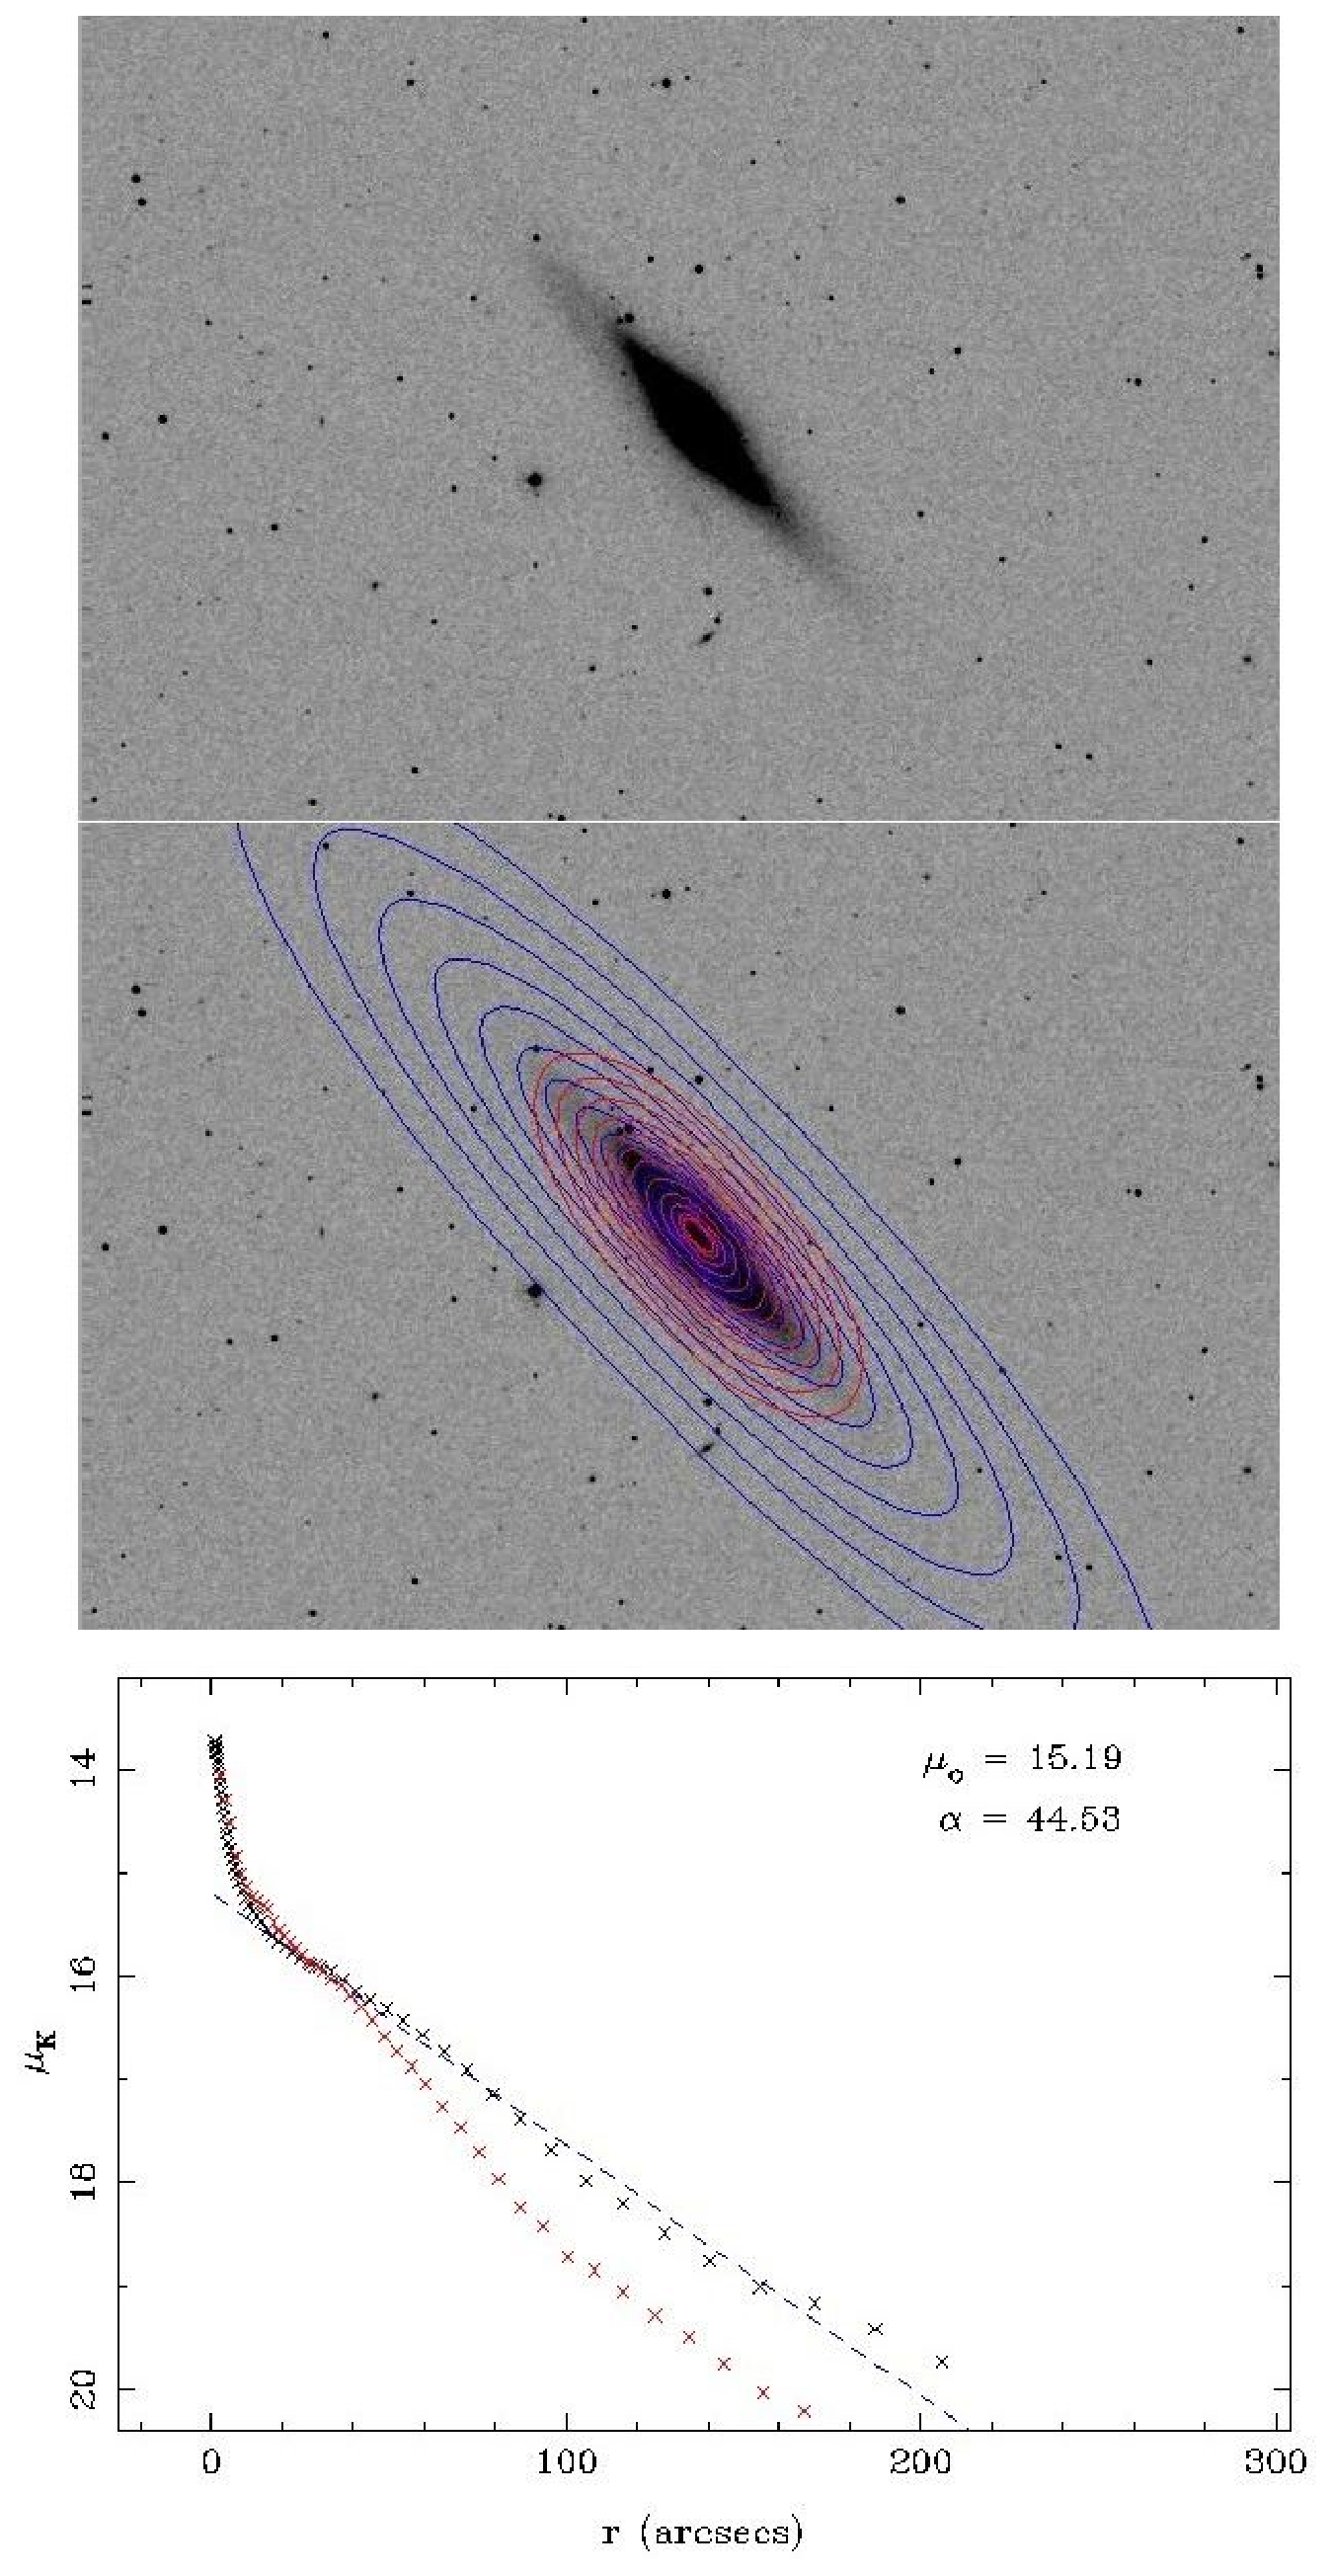
\includegraphics[scale=0.4]{ngc2683_jarrett} \caption{The edge-on Sb galaxy, NGC 2683 selected from the 2MASS Large Galaxy
Atlas. The top and middle panels display greyscale images from the
2MASS $J$ scans. The red ellipses are fits from the 2MASS galaxy
pipeline. The blue ellipses are the resulting fits from this package.
The 2MASS fits clearly fail to follow the flatter isophotes in the
outer regions. This results in an underestimate of these isophote's
intensity values, as seen in the surface brightness profile in the
bottom panel. }
\end{figure}


XML has several key advantages over plain file formats. For one, XML
format allows an endless amount of additional information to be stored
in each file that would not have fit into the standard data plus delimiter
style. For example, calibrating data, such as redshift or photometric
zeropoint, can be stored in each file along with the raw data with
very little increase in file size overhead as the tags handle the
separation. There is no need to reserve space for these quantities
nor is there any problem adding future parameters to the XML format.
Using XML format puts all the reduction data into a single file for
compactness and, in addition, since XML files are plain text files,
there is no problem with machine to machine transfer. The reading
of XML files is not a complication for either compiled or interpreted
languages.

A disadvantage to XML format is that it's clumsy to read. However,
there exist a number of excellent XML editors on the market (for example,
http://www.oxygenxml.com). These allow a GUI interface with an efficient
query system to interact with the XML files. While many users would
prefer to interact with the raw data files in plain text form, in
fact, even a simple editor is GUI window into the bytes and bits of
the actual data on machine hardware. A GUI XML editor is simply a
more sophisticated version of vi or emacs.

\begin{figure}
\centering 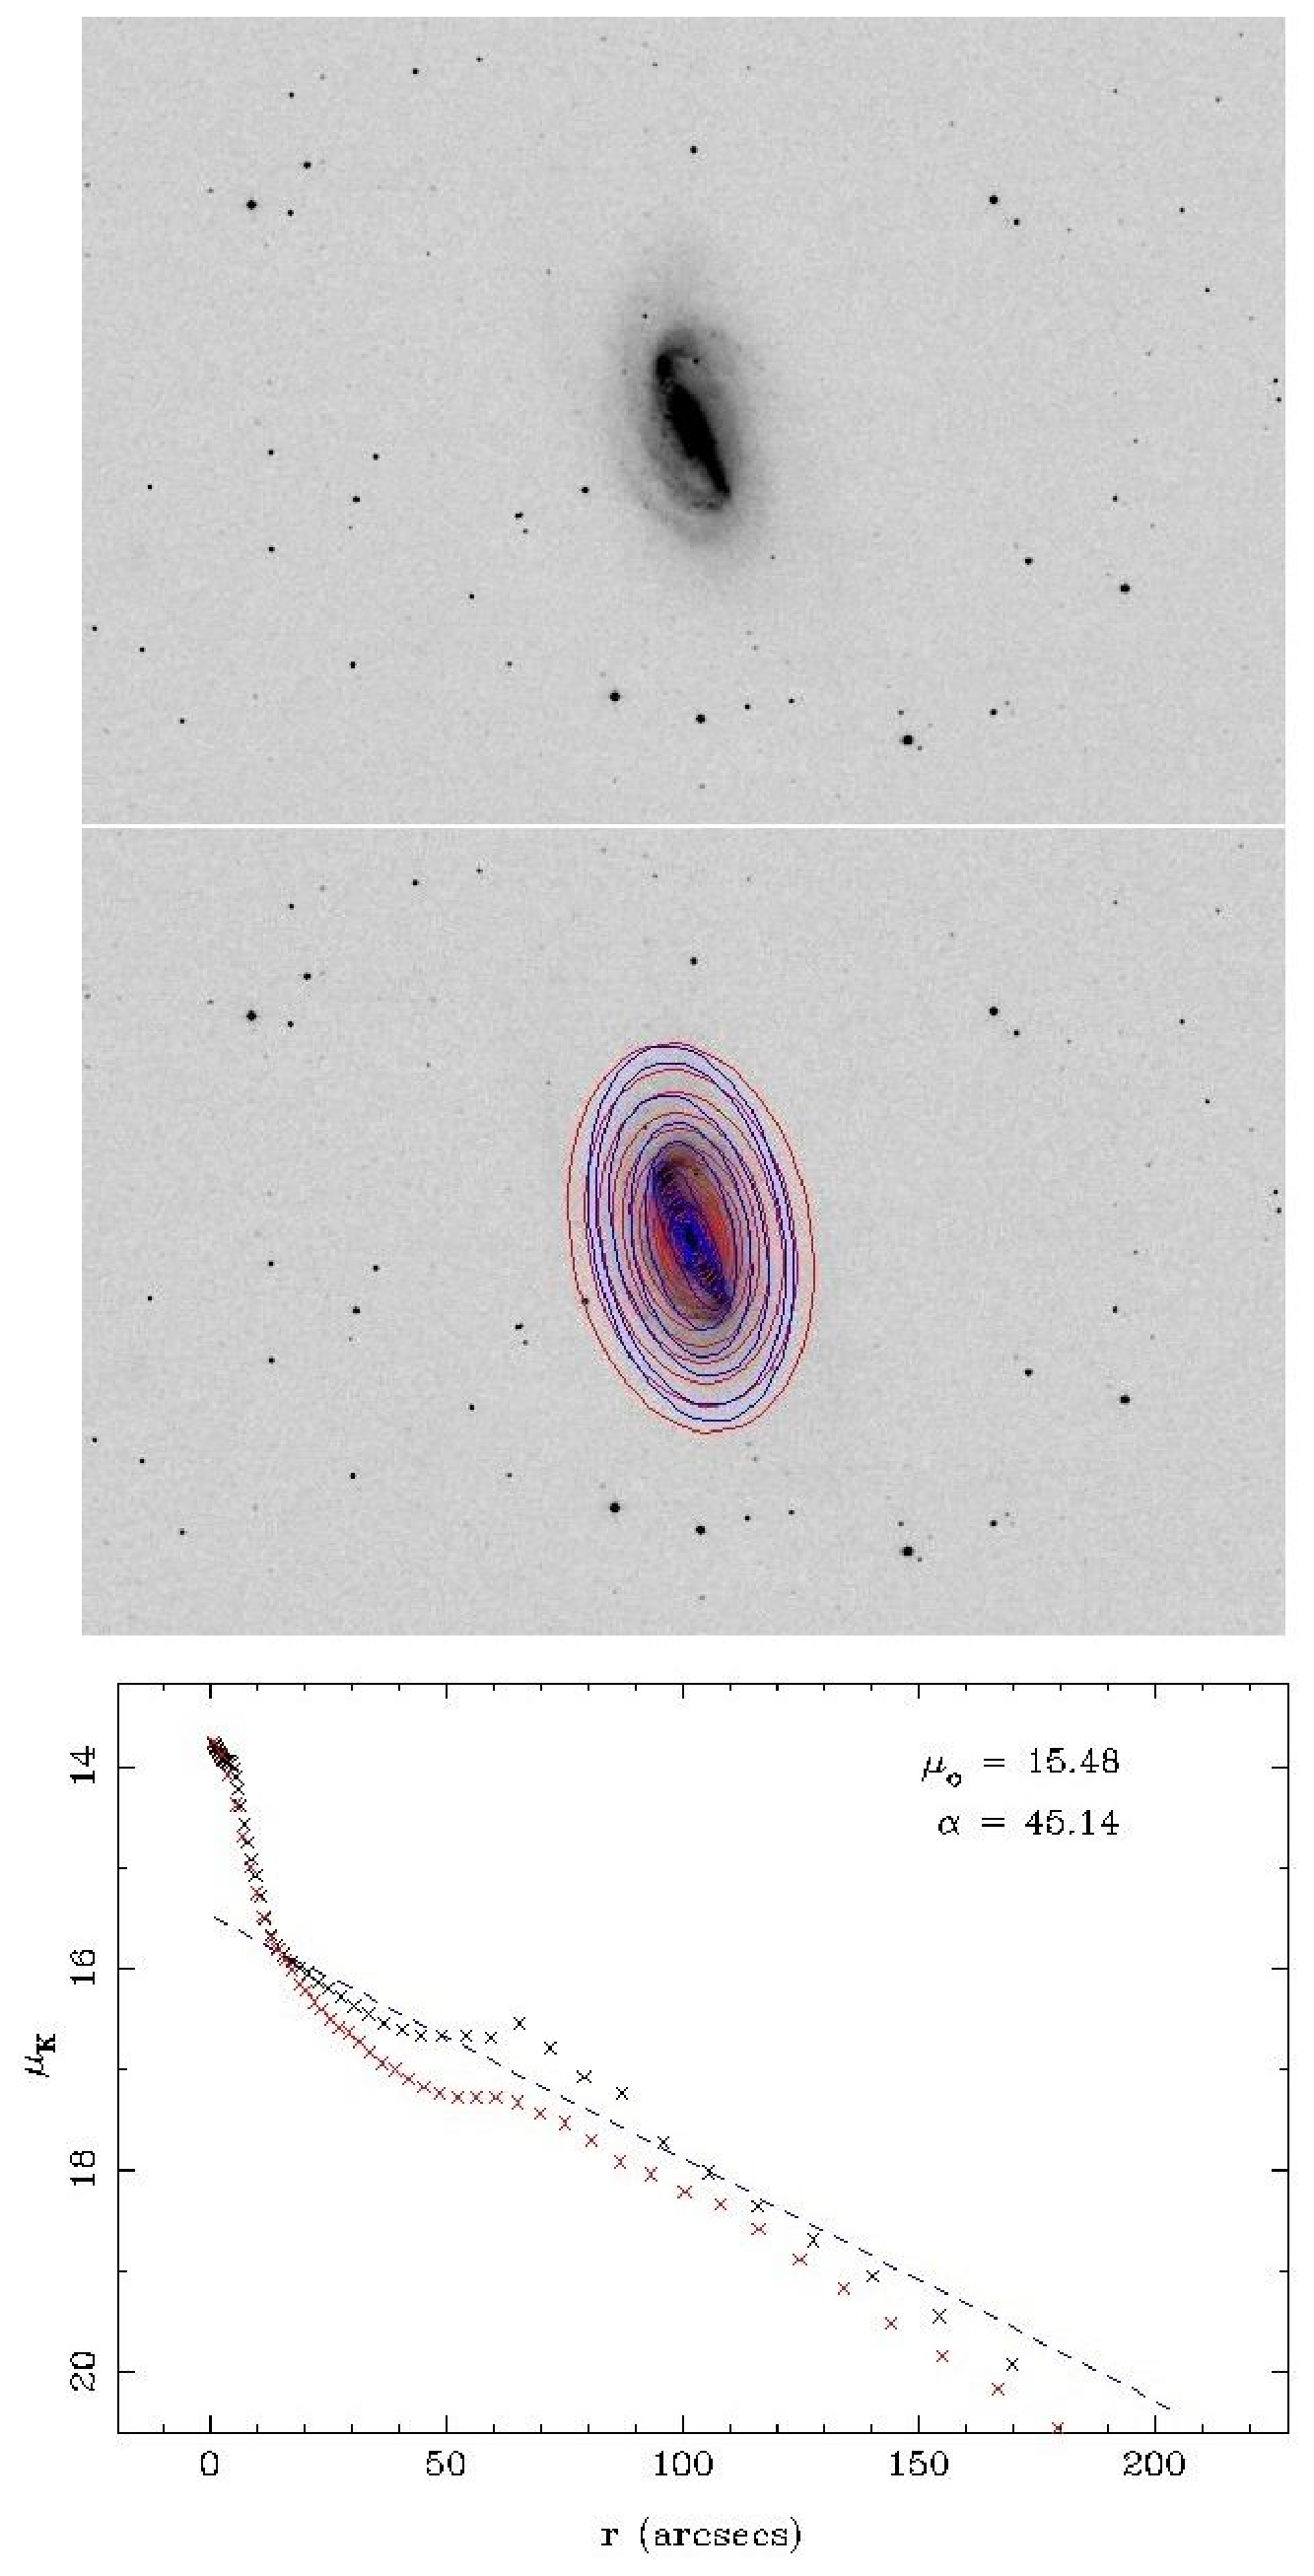
\includegraphics[scale=0.4]{ngc2903_jarrett} \caption{The Sc(s) galaxy, NGC 2903 selected from the 2MASS Large Galaxy Atlas.
The top and middle panels display greyscale images from the 2MASS
$J$ scans. The red ellipses are fits from the 2MASS galaxy pipeline.
The blue ellipses are the resulting fits from this package. The 2MASS
galaxy pipeline failed to follow the isophote twists (i.e. changes
in position angle). This results in an underestimate of these isophote's
intensity values, as seen in the surface brightness profile in the
bottom panel. }
\end{figure}


An additional reason to migrate to XML is a new power that XML data
files bring to data analysis. Many interpreted languages (i.e. Python
and Perl) have an \textit{eval} or \textit{exec} function, a method
to convert XML data into actual variables within the code at runtime
(i.e. dynamically typed). This has a powerful aspect to analysis programs
as one does not have to worry about formats or the type of data entries,
this is handled in the code itself. Dynamical typing introduces a
high level of flexibility to code. In Python, one can convert XML
data (using Python's own XML modules to read the data) into lists
that contain the variable name and value, then transform these lists
into actual code variables using an \textit{exec} command. For example,

\begin{verbatim} for var, value in xmlvars: exec(var+'='+value) \end{verbatim}

\noindent produces a set of new variables in the running code. And
Python's unique try/except processing traps missing variables without
aborting the routine. For example, if the variable 'redshift' exists
in the XML data file then

\begin{verbatim} try: distance=redshift/Ho except: print 'redshift
undefined' distance=stddistance \end{verbatim}

\noindent This same try/except processing also traps overflows and
other security flaws that might be used by a malicious user attempting
to penetrate your server using the XML files. Thus, XML brings a level
of security as well as enhancing your code.

Lastly, another advantage to XML format is the fact that all of the
reduction data (ellipse fitting, aperture photometry, calibration
information, surface photometry) can be combined into a single file,
e.g. galaxy\_name.xml, which can be interrogated by any analysis routine
that understands XML. A simple switch at the end of the reduction
process integrates the data into an XML file for transport, or access
by plotting packages, etc.


\section{A Cautionary Tale, the 2MASS Large Galaxy Atlas}

If you have read this far, and are still awake, this section walks
through the reduction of part of the Revised Shapley-Ames sample (Schombert
2007) taken from the 2MASS database that overlaps the 2MASS Large
Galaxy Atlas (Jarrett \etal 2003). As a cautionary tale to the importance
to doing large galaxy photometry with care, we also offer in this
section a comparison of our technique with the results from an automated,
but much cruder reduction pipeline from the 2MASS project.

Allowing the ellipses to vary from isophote to isophote, not only
in eccentricity, but also in position angle and ellipse center, are
critical to obtaining an accurate description of a galaxy's luminosity
profile. Shown in Figures 10, 11 and 12 are examples of $J$ images
extracted from the 2MASS archives that were part of the Large Galaxy
Atlas (Jarrett \etal 2003). In each case, the 2MASS pipeline calculates
a luminosity profile based on the isophotes around an ellipse from
the mean moments of the whole galaxy. Thus, the fitted ellipses do
not change in axial ratio or position angle and, for most spirals,
this technique will result in an ellipse that is too flat in the core
and, often, too round in the halo regions. If the galaxy has a bar,
this technique will also underestimate the bar contribution, spreading
its light into larger radii ellipses.

\begin{figure}
\centering 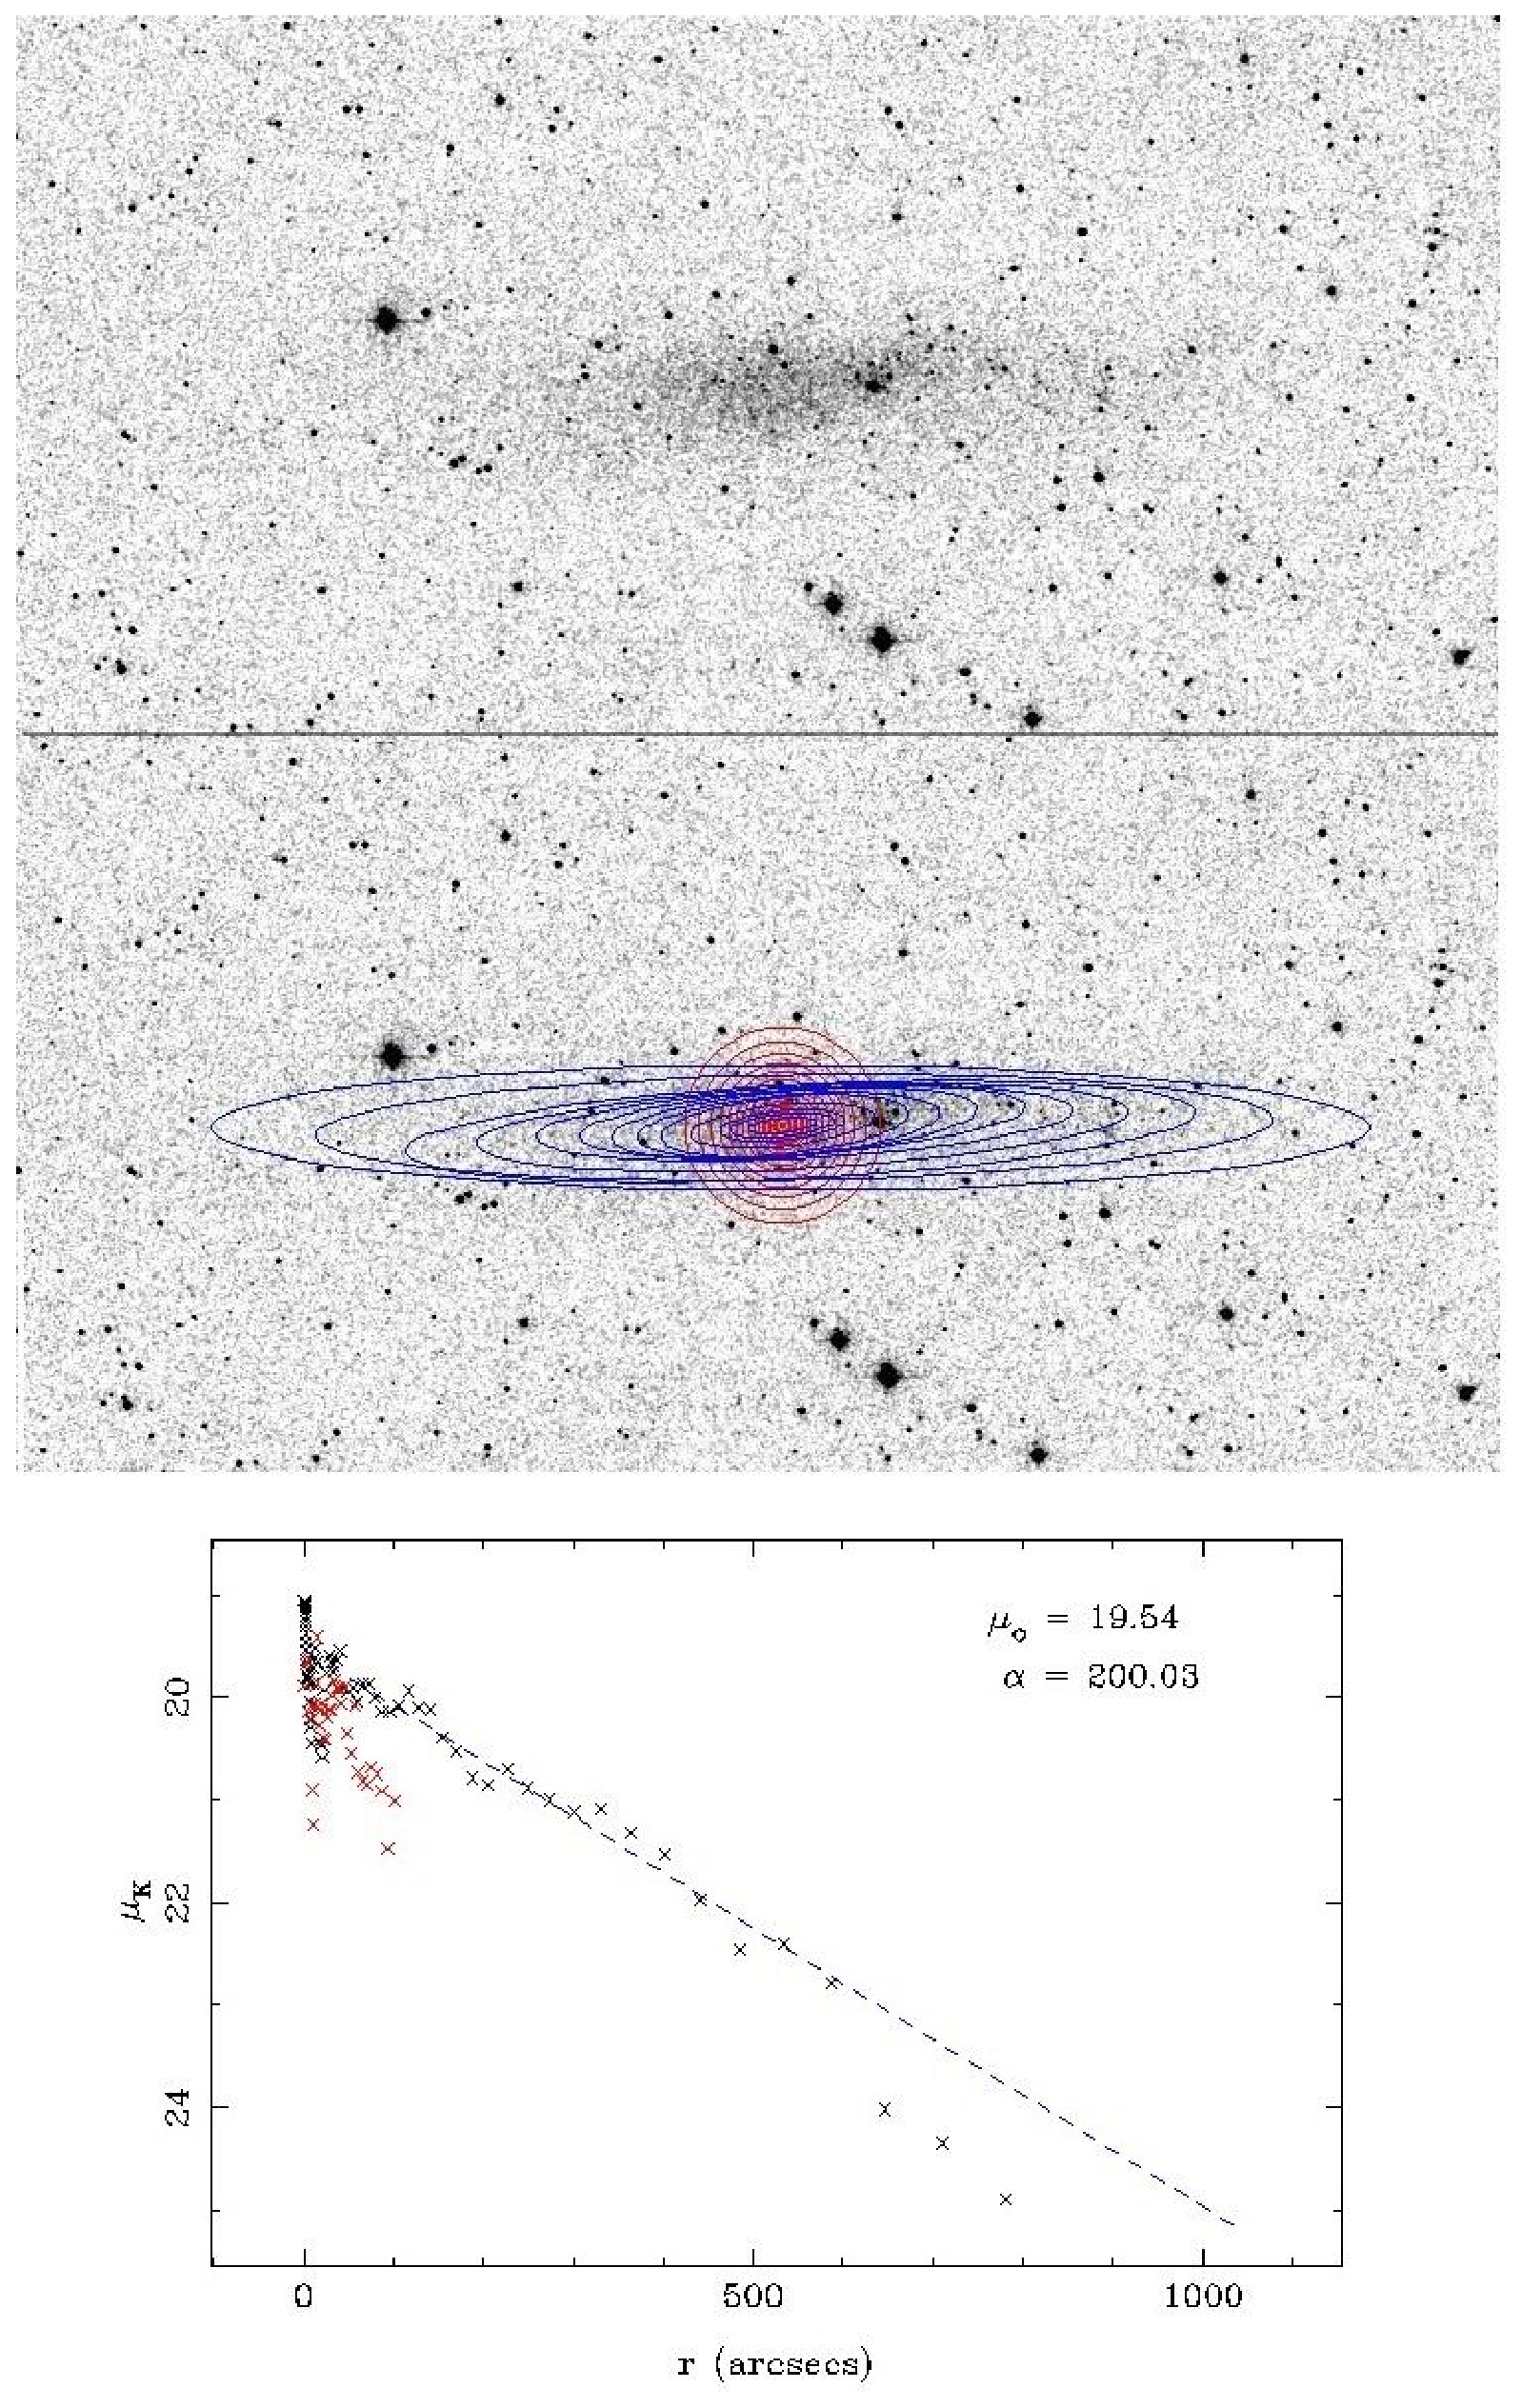
\includegraphics[scale=0.4]{ngc3109_jarrett} \caption{The Sm galaxy, NGC 3109 selected from the 2MASS Large Galaxy Atlas.
The top and middle panels display greyscale images from the 2MASS
$J$ scans. The red ellipses are fits from the 2MASS galaxy pipeline.
The blue ellipses are the resulting fits from this package. The 2MASS
galaxy pipeline, for some strange reason, assumed a circular shape
to was is clearly an elongated galaxy. This results in an underestimate
of these isophote's intensity values, as seen in the surface brightness
profile in the bottom panel. }
\end{figure}


Given that the light is averaged around the ellipse, this effect may
be minor if the galaxy is fairly smooth and uniform. However, galaxies
that are smooth and regular are a minority in the local Universe.
For the three examples, shown in Figure 10, 11 and 12, the 2MASS fits
consistently underestimate the amount of disk light per isophote,
as seen in comparison to the luminosity profile determined from the
raw data using the ARCHANGEL routines. This, in turn, results in fitted
central surface brightnesses that are too bright in central surface
brightness, and fitted disk scale lengths that are too shallow. In
fact, for 49 galaxies in common between the near-IR RSA sample (Schombert
2007) and the 2MASS Large Galaxy Atlas, Figure 13 displays the difference
between the fitted disk scale lengths ($\alpha$) and the difference
between the fitted disk central surface brightness ($\mu$). Given
the typical $\alpha$'s, the error in 2MASS fits corresponds to a
50\% error in a galaxy's size. Likely, errors in the central surface
brightness fits averages around 0.5 mags. Thus, not using the proper
reduction technique not only increases the noise in the measured parameters,
but produces a biased result.

\begin{figure}
\centering 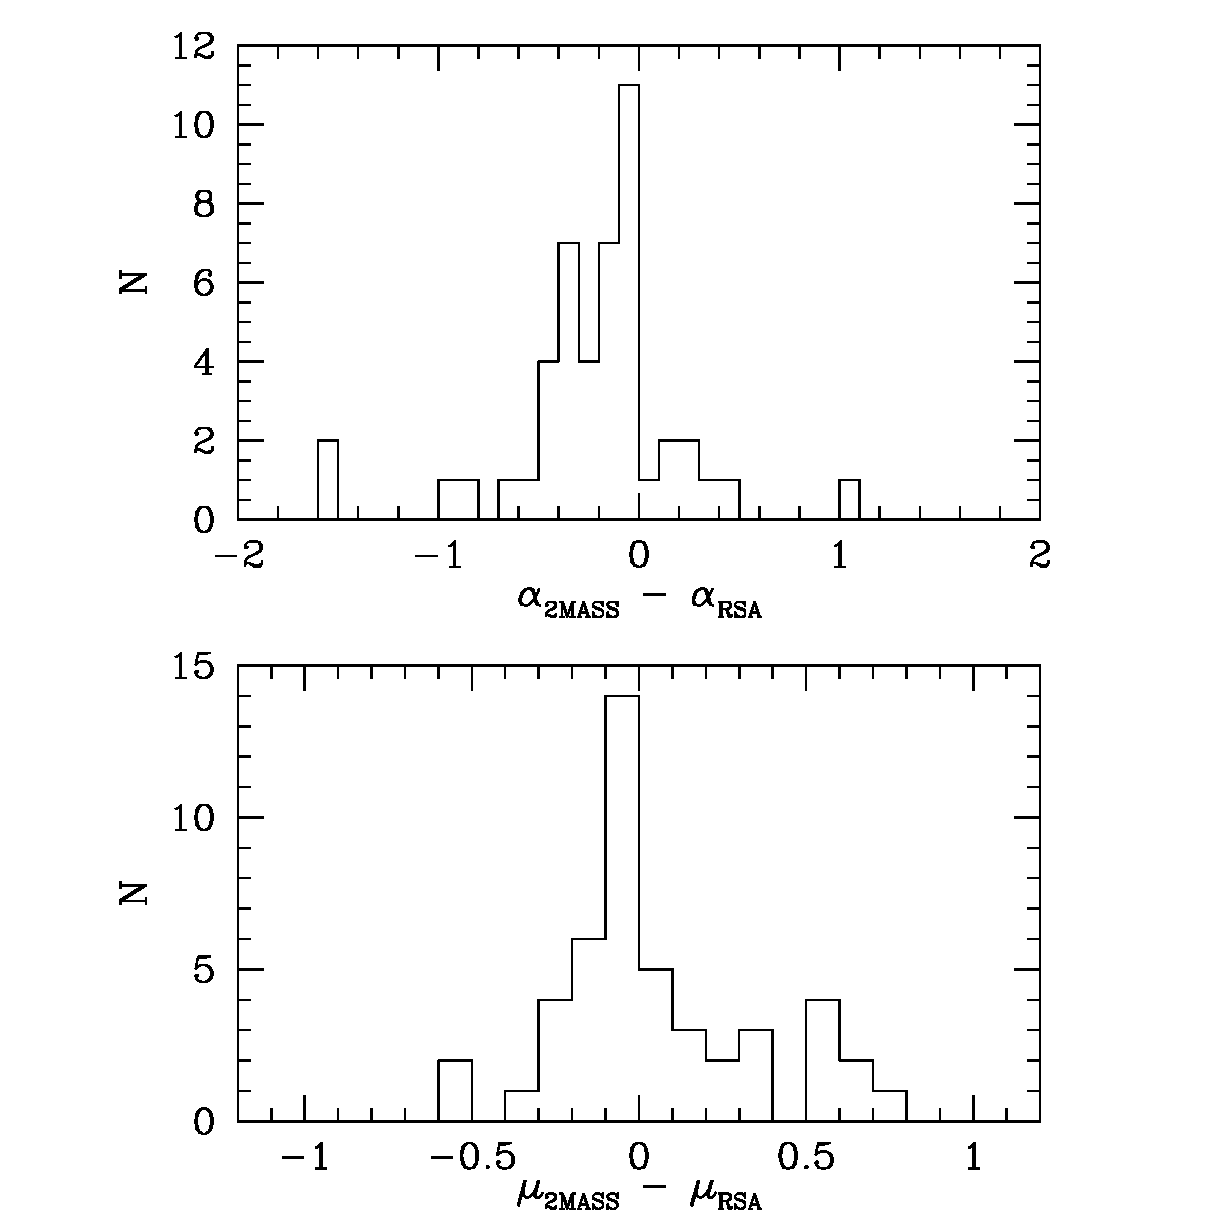
\includegraphics[width=17cm]{hist_fig} \caption{Comparison histograms for 49 galaxies common between the 2MASS Large
Galaxy Atlas and the new near-IR 2MASS RSA dataset. The top panel
displays difference between disk scale lengths ($\alpha$) from fits
of an exponential law to 2MASS surface photometry versus this package's
surface brightness reduction. The bottom panel displays the difference
in fitted center surface brightnesses between the 2MASS profiles and
the new RSA sample. Typically, the 2MASS pipeline overestimates the
eccentricity (too round) which results in smaller scale lengths and
brighter central surface brightnesses. }
\end{figure}



\section{Network Tools}

One of the more powerful modules to the Python language is the $urllib$,
the module that allows Python scripts to download any URL address.
If address is a web page, there also exist several addition modules
that parse HTML and convert HTML tables into arrays. This means a
simple script can be written to pull down a web page, parse it HTML
and extract a data into table format. And, on top of this procedure,
the information could be then be used into a standard GET/POST web
form used by many data archives.

As an example, the package contains \textit{dss\_read}, a script that
takes the standard name for a galaxy, queries NED for its coordinates
and then goes to the DSS website and extracts the PSS-II image of
the galaxy. While this sounds like a computationally intense task,
in fact the script is composed of 49 lines. The downside to this network
power is, of course, the possibility of abuse. Unrestricted application
of such scripts will overload websites and given network speeds, the
typical user doesn't need their own personal digital sky at their
home installation.

Lastly, various archives, in order to slow massive downloads, have
an ID/password interface. To penetrate these sites requires the \textit{mechanize}
module which simulates the actions of a brower, following links, parsing
ID's and passwords and handling cookies. While these avatars are simple
to build, the wise usage of them remains a key challenge for the future.


\section{Package Summary}

The fastest way to learn a data reduction process is to jump in and
try it. To this end, the tarball contains all the images discussed
in this document, and several test images with known output. This
allows the user to practice on images where the final results are
known. Thus, we encourage the readers to download, compile and run!
Tarballs are found at http://abyss.uoregon.edu/$\sim$js/archangel.

Another option, for the user who doesn't wish to set-up the package
on their own system (or perhaps only has a handful of galaxies to
reduce), is the client/server version of this package available at
http://http://abyss.uoregon.edu/$\sim$js/nexus (see Figure 14). Although
more limited in its options, the web version has the advantage of
speed (it's run on a Solaris Sun Blade) and a fast learning curve.

\begin{figure}
\centering 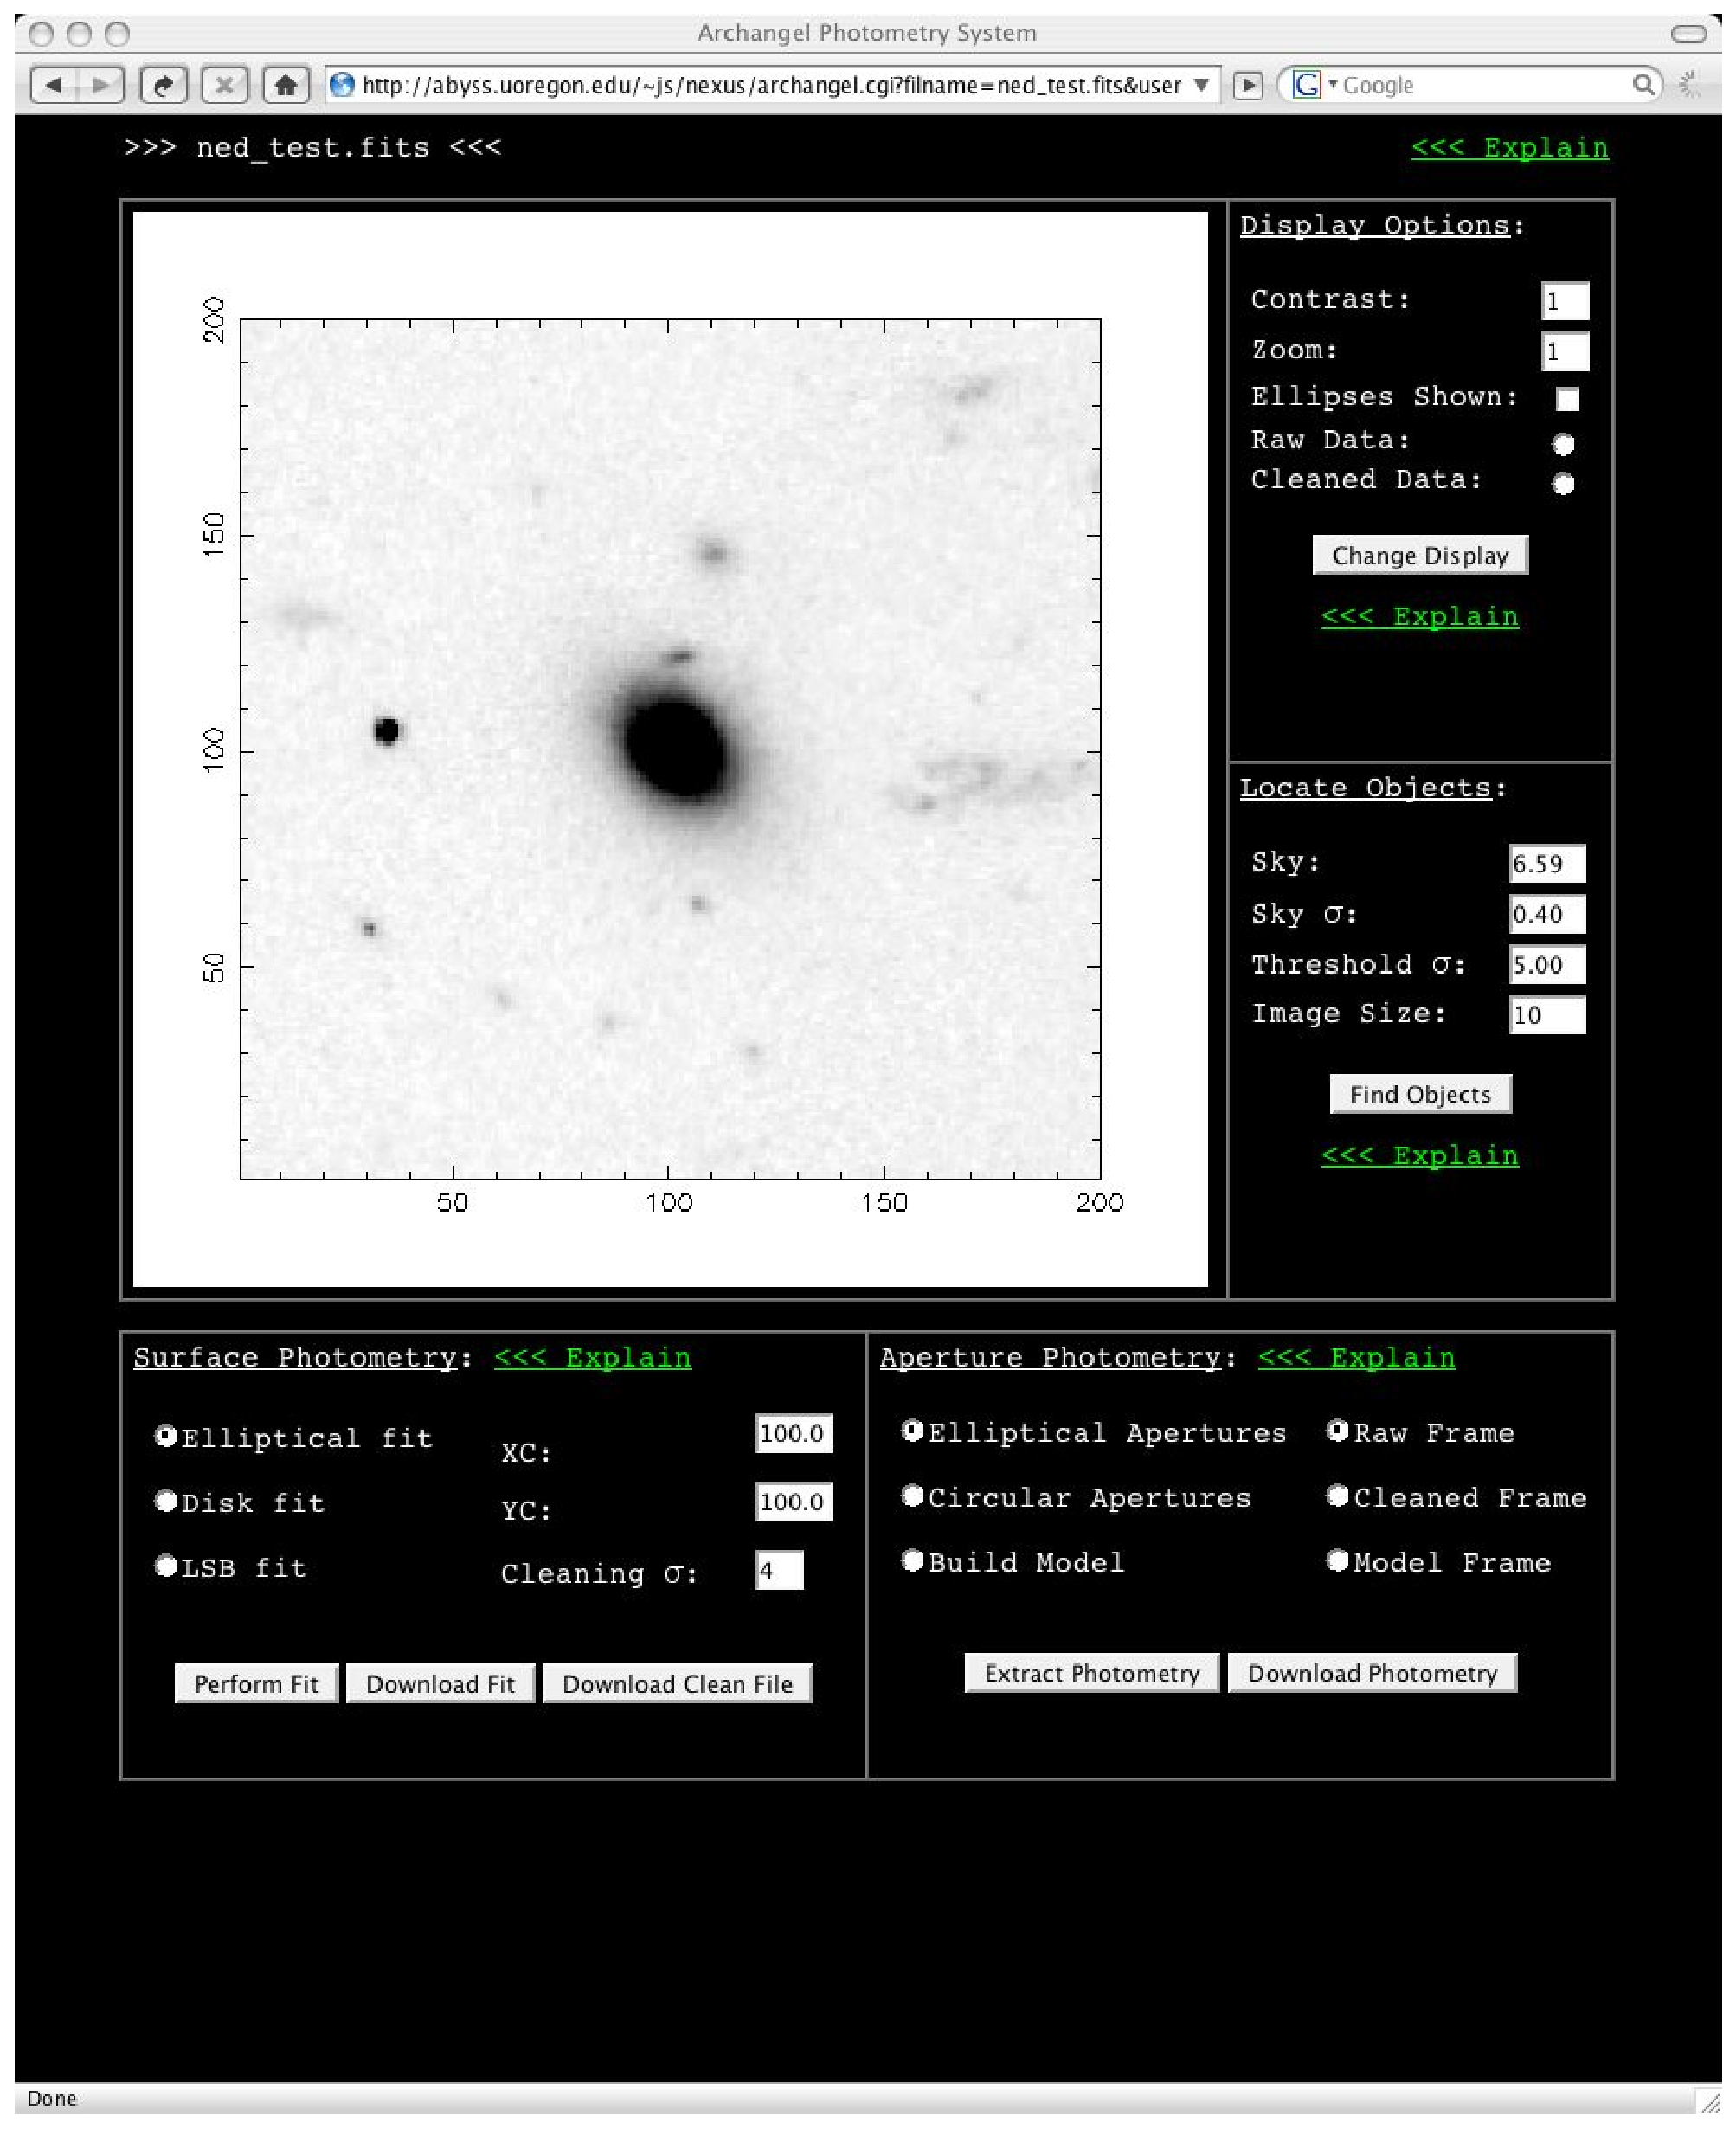
\includegraphics[scale=0.4]{nexus} \caption{A snapshot of the client/server version of this package (using Firefox
on a Mac OS X system). The ability to fit ellipses and perform aperture
photometry exists, as well a crude graphic interface to explore the
isophotal quality. }
\end{figure}


As to the future, a number of tools need to be added to this package.
For example, quantitative morphology uses the concentration and asymmetry
indices to parameterize a galaxy's global structure. While these values
are easy to extract from small angular size objects, they are a challenge
for large systems. Yet, a detailed comparison of these values to visual
morphology is a key step in understanding quantitative morphology
at higher redshifts. However, in order get the current tools out to
the community, the package is frozen. Additional tools will be added
to the package website as, in order of priority, 1) needed by the
PI to meet various science goals, 2) requested by outside users to
obtain their science goals, and 3) requested by outside users as possible
new computational areas to explore. As with all evolving software,
an interested user should contact the author to see where future directions
lie (js@abyss.uoregon.edu).


\acknowledgements{}

This project was funded by Joe Bredekamp's incredible NASA's AIRS
Program. I am grateful to all the suggestions I have gotten from AIRS
PI's at various workshops and panel reviews. The program is a mixed
of technology plus science types and is one of NASA's true gems for
innovative research ideas.
\begin{thebibliography}{References}
\bibitem[Burstein et al.(1987)]{1987ApJS...64..601B} Burstein, D.,
Davies, R.~L., Dressler, A., Faber, S.~M., Stone, R.~P.~S., Lynden-Bell,
D., Terlevich, R.~J., \& Wegner, G.\ 1987, \apjs, 64, 601

\bibitem[Cawson et al.(1987)]{1987MNRAS.224..557C} Cawson, M.~G.~M.,
Kibblewhite, E.~J., Disney, M.~J., \& Phillipps, S.\ 1987, \mnras,
224, 557

\bibitem[Graham & Driver(2005)]{2005PASA...22..118G} Graham, A.~W.,
\& Driver, S.~P.\ 2005, Publications of the Astronomical Society
of Australia, 22, 118

\bibitem[Jarrett et al.(2003)]{2003AJ....125..525J} Jarrett, T.~H.,
Chester, T., Cutri, R., Schneider, S.~E., \& Huchra, J.~P.\ 2003,
\aj, 125, 525

\bibitem[Jedrzejewski(1987)]{1987MNRAS.226..747J} Jedrzejewski, R.~I.\ 1987,
\mnras, 226, 747

\bibitem[Schombert & Bothun(1987)]{1987AJ.....93...60S} Schombert,
J.~M., \& Bothun, G.~D.\ 1987, \aj, 93, 60

\bibitem[de Vaucouleurs(1977)]{1977ApJS...33..211D} de Vaucouleurs,
G.\ 1977, \apjs, 33, 211

\end{thebibliography}
\appendix
%dummy comment inserted by tex2lyx to ensure that this paragraph is not empty



\section{Package Management}

This package is a combination of FORTRAN and Python routines. The
choice of these languages was not arbitrary. Python is well suited
for high level command processing and decision making. It is a clear
and expressive language for text processing. Therefore, its style
is well suited to handling file names and data structures. Since it
is a scripting language, it is extremely portable between OS's. Currently,
every flavor of Unix (Linux, Mac OS X and Solaris) comes packaged
with Python. In addition, there is a hook between the traditional
astronomy plotting package (PGPLOT) and Python (called ppgplot), which
allows for easy GUI interfaces that do not need to be compiled.

The use of FORTRAN is driven by the fact that many of the original
routines for this package were written in FORTRAN. For processing
large arrays of numbers, C++ provides a faster routine, but current
processor speeds are such that even a 2048x2048 image can be analyzed
with a FORTRAN program on a dual processor architecture faster than
the user can type the next command. STScI provides a hook to FITS
formats and arrays (called pyfits and numarray), but Python is a factor
of 100 slower than FORTRAN for array processing.

Currently there are three FORTRAN compilers in the wild, g77, gfortran
and g95. The routines in this package can use any of these compilers
plus a version of Python greater than 2.3. CFITSIO is required and
avaliable for all OS's from its GSFC website. The Python libaries
pyfits and numarray are found at STScI's PyRAF website. For any graphics
routines, the user will need a verson of PGPLOT and install ppgplot
as a Python library. The ppgplot source is avaliable at the same website
as this package. The graphics routines are only needed for data inspection,
the user should probably develop their own high-level graphics to
match their specifics. In the directory /util one can find all the
Python subroutines to fit 1D data surface or aperture photometry.
The examples in this manual will guide you in constructing your own
interface.

Lastly, the output data files for this package are all set in XML
format. This format is extremely cumbersome and difficult to read
(it is basically an extension of the HTML format that web browsers
use). However, a simple command line routine is offered ($xml_{a}rchangel$)
that will dump or add any parameter or array out of or into a XML
file.


\section{Core Analysis Routines}

To go from a raw data frame containing a galaxy image to a final stage
containing ellipse fits, surface photometry, profile fits and aperture
values requires three simple scripts, \textit{profile}, \textit{bdd}
and \textit{el}. The scripts \textit{profile} and \textit{el} are
automatic and can be run as batch jobs. \textit{bdd} is an interactive
routine to fit the surface photometry and is a good mid-point to study
the results of the ellipse fitting. In a majority of cases, the user
simply needs to run those three scripts with default options to achieve
their science results.

Note that command -h will provide a short summary of the commands
usage.

\noindent \textit{sky\_box}: \begin{verbatim} Usage: skybox option
filename boxsize prffile options: -h = this message -f = first guess
of border -r = full search, needs boxsize and prffile -t = full search,
needs boxsize -c = find sky for inner region (flats) needs x1,x2,y1,y2
boundarys Output: 1st mean, 1st sig, it mean, it sig npts, iterations
\end{verbatim}

\noindent {$efit$}:\begin{verbatim} Usage: efit option filename
outputfile otherops

Ellipse fitting routine, needs a standard FITS file, output in .prf
file format (xmlarchange converts this format into XML) options: -h
= this mesage -v= output each iteration -q = quiet -xy = use new xc
and yc -rx = max radius for fit -sg = deletion sigma (0=no dets) -ms
= min slope (-0.5) -rs = stopping radius -st = starting radius when
deleting, output FITS file called filename.jedsub\end{verbatim}

\noindent {$prf\_smooth$}: \begin{verbatim} Usage: prfsmooth option
prffilename

parameter \#6 set to -1 for cleaned ellipse, 0 for unfixable ones

options: -x = delete unfixable ones -s = spiral, low smooth -d = neutral
smooth -q = quick smooth \end{verbatim}

\noindent {$prf\_edit$}: \begin{verbatim} Usage: prfedit filename

visual editor of isophote ellipses output from efit

note: needs a .xml file, works with cleaned images

cursor commands: r = reset display z = zoom in c = change cont x =
flag ellipse/lum point t = toggle wd cursor o = clean profile q =
exit h = this message \end{verbatim}

\noindent {$probe$}: \begin{verbatim} Usage: probe option masterfile

quick grayscale display GUI

options: -f = do this image only -m = do file of images

cursor commands: / = abort q = move to next frame c = contrast r =
reset zoom z = zoom t = toggle ellipse plot p = peek at values a,1-9
= delete circle b = delete box \end{verbatim}

\noindent {$bdd$}: \begin{verbatim} Usage: bdd options filename

quick surface photometry calibration and fitting GUI

options: -h = this message -p = force sfb rebuild

window \#1 cursor commands: c = contrast control r = reset boundaries
z = zoom on points x = delete point s = set sky (2 hits) i = show
that ellipse / = write .sfb file q = abort

window \#2 cursor commands: x = erase point d = disk fit only m =
erase all min pts f = do bulge+disk fit u = erase all max pts e =
do r{*}{*}1/4 fit only b = redo boundaries p = toggle 3fit/4fit q
= abort r = reset graphics / = write .xml file and exit

\end{verbatim}

\noindent \textit{xml\_archangel}: \begin{verbatim} xmlarchangel
op filename element data

add or delete data into xml format -o = output element value or array
-d = delete element or array -a = replace or add array, array header
and data is cat'ed into routine -e = replace or add element -c = create
xml file with root element -k = list elements, attributes, children
(no data) \end{verbatim}

\noindent {$el$}: \begin{verbatim} Usage: el options cleanedfile

script that takes cleaned FITS file and fills in NaN pixels from efit
isophotes, then does elliptical apertures on resulting .fake file

options: -v = verbose \end{verbatim}

\noindent {$asymptotic$}: \begin{verbatim} Usage: asymptotic xmlfile

simply GUI that determines asymptotic fit on integrated galaxy mag,
delivers mag/errors from apertures and curve of growth fit into XML
file

cursor commands: r = reset a = adjust lum for better fit f = linear
fit x,1,2,3,4 = delete points z = set profile extrapolation point
/ = exit b = change borders \end{verbatim}
\end{document}
